\documentclass[11pt]{article}
\usepackage[margin=1.1in]{geometry}
\usepackage{amsmath,amssymb,amsthm,mathtools,booktabs,array,longtable}
\usepackage[T1]{fontenc}
\usepackage{lmodern}
\usepackage{microtype}
\usepackage{enumitem}
\usepackage{url}
\usepackage{placeins}
\usepackage{tikz}
\usetikzlibrary{arrows.meta,positioning}
\usepackage[square]{natbib}
\usepackage[hidelinks]{hyperref}
\hypersetup{pdftitle={Alp\"oge's Certified Lean Derivation Does Not Prove the Riemann Hypothesis: Granting Every Check, the Hypothesis Follows from a Premise Stronger Than Itself},pdfauthor={Parker Emmerson (Yaohushuason)}}
\makeatletter\g@addto@macro{\UrlBreaks}{\do\_}\makeatother
\emergencystretch=2em

\newtheorem{theorem}{Theorem}[section]
\newtheorem{proposition}[theorem]{Proposition}
\newtheorem{corollary}[theorem]{Corollary}
\newtheorem{lemma}[theorem]{Lemma}
\theoremstyle{definition}
\newtheorem{definition}[theorem]{Definition}
\theoremstyle{remark}
\newtheorem{remark}[theorem]{Remark}

\newcommand{\re}{\operatorname{Re}}
\newcommand{\RHraw}{\mathsf{RH}_{\mathrm{raw}}}
\newcommand{\C}{\mathbb C}
\newcommand{\Hp}{\mathbb H}
\newcommand{\St}{\mathbb S}
\DeclareRobustCommand{\lean}[1]{{\renewcommand{\_}{\textunderscore\allowbreak}\texttt{#1}}}
\newcommand{\True}{\lean{True}}
\newcommand{\False}{\lean{False}}


\title{Alp\"oge's Certified Lean Derivation\\ Does Not Prove the Riemann Hypothesis:\\[4pt] \large Granting Every Check, the Hypothesis Follows\\ from a Premise Stronger Than Itself}
\author{Parker Emmerson (Yaohushuason)\\[2pt]
\small Independent Researcher\\
\small ORCID 0009-0007-1288-3292\\
\small \texttt{Parkeremmerson@icloud.com}}
\date{23 November 2026\\[2pt]\small Version 5}

\begin{document}
\maketitle


\begin{abstract}
On 20 November 2026 Levent Alp\"oge released a note stating his belief that he has proved the Riemann hypothesis, with an archive for the Lean theorem prover in which the argument is formalized ``without assumptions,'' and on 21 November the Lean and Mathlib communities certified the statement and the derivation. This note establishes that the certified derivation does not prove the Riemann hypothesis. It derives the sentence of the hypothesis in the prover's rules, and in three senses a derivation in those rules is not a proof of the hypothesis. First, it does not establish that the hypothesis holds of the whole numbers. Outright it establishes that a whole number at which the law failed would yield a derivation of \False{} in the rules; the law itself follows from one premise, its sponsor: the consistency of the rules. That sponsor is a stronger statement than the hypothesis; the rules leave it underived if it holds, and they derive that they are right about this law exactly when they derive the law (L\"ob, 1955); every derivation of it elsewhere rests on a further sponsor of the same kind, along the progression of stronger systems that Turing described in 1939; and none of the four checks of the certification tests it. Second, it is not a proof from the zeta series: on the half-plane where the series converges the sentence receives both truth values, and the derivation takes the continuation, the excluded middle and clauses that write ``0'' from the rules. Third, it is not a certified proof in the set theory to which the word ``proved'' ordinarily refers: the rules derive a statement of arithmetic that this set theory leaves underived. The note then reads the certified derivation against the published list of the names in the exported proof. The absence of zeros is produced at one step, by the refutation of a supposed zero of a continued function; the derivation exhibits no zero; among its premises is a theorem whose constant is asserted through a division on a supposed real zero (Siegel, 1935); and the condition that the archive names for geometry is filled by the one that holds of every object, the condition that asks for a geometric witness being absent from the exported proof. On 23 November 2026 the public record still listed two runs of the check as unfinished. Statements about the rules are checked in Lean 4.33.1; a notebook reproduces the readings.
\end{abstract}

\noindent\textbf{Keywords:} Riemann hypothesis; formal proof; Lean theorem prover; Mathlib; zeta series; analytic continuation; excluded middle; incompleteness; consistency; L\"ob's theorem; Turing progression; Markov's principle; completion by clause


\section{Introduction}\label{sec:intro}

The certified derivation of the Riemann hypothesis does not prove the Riemann hypothesis. That is the statement of this note, and the note says in what senses it holds.

The certificate of 21 November 2026 is the certificate of a derivation: a finite term in the rules of the Lean prover whose type is the sentence of the hypothesis, accepted by programs. With the certification as its sponsor that derivation exists, and the note does not dispute it. A derivation in those rules is not a proof of the hypothesis, in three senses that the word ``proved'' carries in the claim that the hypothesis has been proved.

\emph{It does not establish that the hypothesis holds of the whole numbers.} What the certified derivation establishes outright, about the whole numbers, is one conditional: a whole number at which the law of the hypothesis failed would yield a derivation of \False{} in the prover's rules (Theorem~\ref{thm:outright}). The law itself holds on a sponsor, the consistency of the rules, and that sponsor is a stronger statement than the hypothesis, is left underived by the rules, and is tested by none of the checks of the certification (Theorems~\ref{thm:stronger} and~\ref{thm:lob}, Proposition~\ref{prop:checks}).

\emph{It is not a proof from the zeta series.} The series is the datum from which the hypothesis is formed. It has a sum on the half-plane of the complex numbers $s$ with real part above $1$, and the zeros of which the hypothesis speaks lie outside that half-plane, at places where the series has no sum and a further stipulation, analytic continuation, writes the values. From the series on its half-plane the sentence of the hypothesis receives both truth values, one at some completions of the series and the other at others (Theorem~\ref{thm:both}). A derivation from the series alone therefore does not exist, and the certified derivation is a derivation from further premises (Corollary~\ref{cor:notfrom}). The note reads those premises from the certified archive: the continuation, the excluded middle, and clauses that write ``0'' where a rule supplies no value. It reads, too, the one step at which the absence of zeros is produced, a refutation of a supposed zero (Proposition~\ref{prop:junction}).

\emph{It is not a certified proof in set theory.} In mathematics the word ``proved'' ordinarily refers to the set theory of Ernst Zermelo (1871--1953) and Abraham Fraenkel (1891--1965) with the axiom of selection (classically, the axiom of choice). The prover's rules derive a statement of arithmetic that this set theory leaves underived, so a derivation in the rules is not thereby a derivation in it, and no check of the certification concerns a derivation in it (Proposition~\ref{prop:beyond}).

Theorem~\ref{thm:notproof} collects the three. The note that announced the archive states its author's belief that the hypothesis is proved, and describes the formalized argument with the words ``without assumptions''; the joint statement of the Lean and Mathlib communities certifies that the statement and the proof are correct. Those words cover the derivation. The first of the three senses holds of every law of the whole numbers that the rules derive, and the note says so; the second and the third are particular to the hypothesis and to the prover.

\subsection{The derivation and its certification}

The Riemann hypothesis, which Bernhard Riemann (1826--1866) stated in 1859, says that every non-trivial zero of the zeta function, a point at which the function takes the value ``0'' other than the negative even integers, has real part $\tfrac12$~\citep{riemann}. On 20 November 2026 Levent Alp\"oge released a four-page note and an archive of source files for the Lean theorem prover~\citep{alpoge,lean4}. The note states its author's belief that he has, working with the language model Claude, found a proof of the hypothesis, and that the argument has been formalized in Lean without assumptions. The archive holds 175{,}187 Lean files with 17{,}374{,}215 lines (Supporting Information, Part~1). It is pinned to version~4.33.1 of the prover and to one commit, a recorded state, of the Mathlib library, the prover's library of mathematics~\citep{mathlib}. Its file \lean{Main.lean} states five theorems. The first, \lean{riemannHypothesis}, has for its statement the library's own definition \lean{RiemannHypothesis}; the second states the same in the archive's wording; and the other three state the corresponding results for the $L$-functions of the characters of Peter Gustav Lejeune Dirichlet (1805--1859), whose definition Section~\ref{sec:route} recalls.

On 21 November 2026 the Lean and Mathlib communities issued a joint statement, endorsed by the Lean FRO and the Mathlib Initiative, which certifies that the statement and the proof are correct~\citep{leanblog}. The statement reports four checks: that the statement proved is the library's \lean{RiemannHypothesis}, a definition vetted by experts in the prover and in number theory; that the archive compiles; that the theorem proved matches that statement, which two comparison tools confirmed; and that the exported proof is accepted by the prover's kernel and by several independently written checkers. The verification record kept by Andrew Sutherland reports that the five theorems rest on three axioms, \lean{propext}, \lean{Classical.choice} and \lean{Quot.sound}, and on no others~\citep{sutherland}.

\subsection{The question}

This note asks what the certified derivation decides. The question was put before the derivation existed. Two manuscripts by the author, completed earlier in November 2026, asked what a proof of the hypothesis would prove and answered with theorems~\citep{tv,rhp}. Their answer was that the truth value of the hypothesis enters with a clause, the analytic continuation that writes values of the zeta function where its series has none; that the data which form the sentence leave it underivable; and that a classical proof, if one were given, would be a derivation of the content of that clause, delivered as the refutation of a balance. A derivation has now been certified, and the note reads it against that answer.

The reading turns on one distinction. To say that rules \emph{decide} a statement can mean that they assign it a truth value, or that they derive it or its counter-inscription. The prover's rules do the first for every statement and the second for some. The first is the work of clauses that write ``0'' where a rule supplies no value, in the terms of the prover and in its logic. The second is limited by the incompleteness theorem of Kurt G\"odel (1906--1978) of 1931. A statement to which the rules assign a value, while no derivation of that value is in hand, holds the value by a clause. Until 20 November 2026 the Riemann hypothesis, as the library states it, was in that position. With the certification as its sponsor, the archive supplies a derivation. It is a derivation inside the rules that the clauses complete, and it leaves the first answer where it was: the data that form the sentence do not derive it.

The note asks a second question, which the first makes exact: what does the claim that the hypothesis is proved cover? A derivation is a finite object, and that it exists is a fact that programs check. That the derived sentence holds of the whole numbers is a further statement. It follows from the first on the premise that the rules derive no falsehood, and Section~\ref{sec:sponsor} shows that this premise is a stronger statement than the hypothesis, that the rules cannot supply it, and that the certification does not test it. The note does not dispute the derivation. It states what the words that have been used of it cover.

\subsection{Terms and conventions}

The conventions are those of the two manuscripts. The thesis under study is that ``0'' is written by a completion; the note's own voice therefore mentions the term, in quotation marks, where it speaks of the classical inscription. A function $F$ \emph{issues} the value $c$ at $s$ when $F(s)=c$. A value \emph{presents a magnitude} when it has an inverse, a value whose product with it is $1$ (classically, when it differs from $0$). A function $F$ \emph{balances} at $s$ when its value there is the difference of two presented magnitudes that agree (classically, $F(s)=0$), and $s$ is then a \emph{balance point} of $F$; the non-trivial zeros of the zeta function are balance points. A statement is \emph{refuted} when its \emph{counter-inscription} holds, the sentence that the classical language writes as its negation, and a value is \emph{apart from} another when the two differ (classically, $\neq$). Where a classical formula is recast, the classical form follows in parentheses. Each person is dated at first mention, by years of life or by the year of the work cited; each technical term is defined where it first appears; and a theorem names its hypotheses as its \emph{sponsors}. The \emph{tallies} are the whole numbers from $1$ up; the prover's natural numbers begin with ``0.''

The note keeps two words apart. To \emph{derive} a sentence is to produce a derivation of it in stated rules; that a derivation exists is a finite fact, which programs check. To \emph{prove} the hypothesis, in the statement of this note and in the claim that it examines, is to establish it: in the first place, to establish that its law holds at every whole number. Where the note describes the archive, the library or the literature it uses ``proof'' as they do, for a derivation or for the argument beneath a theorem, and the \emph{exported proof} is the name of a file.

\emph{The prover} is Lean, version~4.33.1; \emph{the library} is Mathlib at the commit to which the archive is pinned; \emph{the archive} is the released collection of Lean files; and \emph{the certification} is the joint statement of 21 November 2026.

\subsection{Results}

\begin{enumerate}[leftmargin=2em,itemsep=2pt]
\item \emph{The certified derivation does not prove the hypothesis.} It is a derivation in the prover's rules, and it is not a proof of the hypothesis in three senses: it does not establish outright that the hypothesis holds of the whole numbers, it is not a derivation from the zeta series, and it is not a certified derivation in the set theory to which the word ``proved'' ordinarily refers (Theorem~\ref{thm:notproof}). Outright, the certified derivation establishes that a whole number at which the law of the hypothesis failed would yield a derivation of \False{} in the rules, and nothing more about the whole numbers (Theorem~\ref{thm:outright}). Of the four combinations of ``the law holds'' and ``the rules are consistent'' it excludes one, and the favourable one is confirmed by no finite computation (Proposition~\ref{prop:fourcases}). The sponsor on which the law holds, the consistency of the rules, implies the law and is not implied by it in the rules (Theorem~\ref{thm:stronger}); the rules derive that they are right about the law exactly when they derive the law (Theorem~\ref{thm:lob}); a derivation of the sponsor in a stronger system rests on the consistency of that system, at every step of a progression that no step closes (Theorem~\ref{thm:ladder}); and none of the four checks of the certification tests it (Proposition~\ref{prop:checks}).
\item \emph{The series does not derive the sentence.} The data that form the sentence of the hypothesis, the zeta series on the half-plane where it converges with the class of its completions and the form of the sentence, give the sentence both truth values, and every system of rules sound for them leaves it underived (Theorem~\ref{thm:both}). Complex differentiability selects one completion, at which the sentence is the library's \lean{RiemannHypothesis} (Theorem~\ref{thm:selection}). The certified derivation invokes facts about the selected function that another completion of the same series refutes (Proposition~\ref{prop:laststep}), and it is not a derivation from the formation data (Corollary~\ref{cor:notfrom}).
\item \emph{The route.} Thirty-two links of named calls lead from the final theorem to a windowed criterion of the type of Edmund Landau (1877--1938) and, inside it, to the steps of item~3 (Proposition~\ref{prop:chain}). The criterion turns a one-sided bound for a sum over the prime powers into the absence of zeros (Proposition~\ref{prop:window}). The series enter it through four library identities on the half-plane where they converge, and the zeros are excluded for the continued functions (Proposition~\ref{prop:enters}). The criterion's proof has two halves: one reads a convergent integral of sums over the prime powers, the other begins from a supposed zero and reads the continued function, and they meet at one lemma about positive real numbers (Proposition~\ref{prop:junction}); the clash is made by the place of the supposed zero, since a zero on the line receives the same treatment and meets none (Proposition~\ref{prop:online}). Among the premises of the exported proof is the theorem of Siegel, whose constant is asserted through a division on a supposed real zero that the archive's own conclusion shows to be absent (Proposition~\ref{prop:siegel}).
\item \emph{The clauses.} The prover's terms are completed by clauses that write a value where the rule of an operation supplies none, and the certified sentence is written in these terms (Proposition~\ref{prop:clauses}); the library's own term for the zeta series issues ``0'' at every point of the critical strip (Proposition~\ref{prop:series}). Three steps of the route call a clause, and two of them conclude that a function is integrable from the clause that writes ``0'' as the integral of a function that has none (Proposition~\ref{prop:clausesteps}). That inference, read as a schema, is equivalent to the excluded middle (Theorem~\ref{thm:backward}).
\item \emph{The two completenesses.} In the prover's rules every statement is decided in value (Theorem~\ref{thm:value}). If the rules are consistent, some statement is derived by them in neither form (Theorem~\ref{thm:rosser}); it holds its value by the clause alone (Corollary~\ref{cor:alone}); and the consistency of the rules is such a statement (Theorem~\ref{thm:second}). The sentence of the hypothesis had a value, by one step that uses no property of the zeta function, before any derivation of it (Corollary~\ref{cor:before}).
\item \emph{What is delivered.} The derivation delivers the refutation of a balance, from which the guarded clause of a field gives an inverse (Theorem~\ref{thm:defence}); the passage from the refutation to a presented bound is Markov's principle, and conversely (Theorem~\ref{thm:markov}).
\item \emph{The certification and the certified term.} The rules derive a statement of arithmetic that the standard set theory leaves underived (Proposition~\ref{prop:beyond}). On 22 and on 23 November 2026 the verification record listed two runs of the check as unfinished (Proposition~\ref{prop:state}). The text of the sources contains no option, axiom or declaration that weakens the check or changes the sentence (Proposition~\ref{prop:scan}). The bound that the criterion needs is supplied by the body of the archive. Its lemmas take a condition that the archive's names tie to geometry, and wherever the text supplies that condition by name it is the one defined to hold of every object; of the accounts of this part that were public on 22 November 2026, none is offered by its author as a checked derivation of the bound (Proposition~\ref{prop:bound}). By the published list of the names in the exported proof, the condition that holds of every object and a degenerate model of the archive's type of geometries are in the exported proof, and the condition that asks for a geometric witness, with the declarations that tie a divisor record to a family, is not (Proposition~\ref{prop:compiled}).
\end{enumerate}

\noindent Section~\ref{sec:position} states the position that these results support.


\subsection{Sources and the method of reading}\label{sec:method}

The copy of the archive that was read is the repository of~\citet{mirror}, at the commit named in the Supporting Information. Its README records that it holds the contents of the joined archive without modification and gives the SHA-256 value of the joined archive, a fingerprint computed from the contents of the file, which is the value that the verification record gives~\citep{sutherland}. The prover's core library was read at the tag of version~4.33.1, and Mathlib at the commit named in the archive's manifest, the file that lists the versions on which the archive depends. \emph{Reading} means reading the text of declarations. The prover was not run on the archive for this note: every statement of the note of the form ``the archive derives \dots'' has the certification as its sponsor, and the note adds to the certification what the text of the declarations shows. A \emph{link} is the occurrence of the name of one declaration in the text of another, and the \emph{route} is the chain of links that leads from the final theorem down to the steps named in Section~\ref{sec:route}. That a link holds is a fact about text; the prover's own computation of what a theorem depends on was not run here. Counts of words in the archive are counts of text and are reported as such. For this version the names are also looked up in the list of the 1{,}484{,}733 declarations, constructors and recursors of the exported proof of \lean{Main.lean} that~\citet{dixit} published with an independent reproduction of the build, one line for each, with its kind and its full name; the independent run of~\citet{lipponen} counts 1{,}478{,}243 constants for the five theorems and 1{,}478{,}219 for \lean{riemannHypothesis} alone. A name is \emph{in the exported proof} when it is a line of that list. That a name is in the list, or is not, is a fact about the published file, which has the two reproductions as its sponsors; the account of~\citet{vincit}, read from the Lean source, was consulted for the same part. The state of the certification is read from the verification record and from the notes of the checkers' repository as they stood on 22 November 2026, with the record read again on 23 November~\citep{sutherland,leannotes}, and the announced argument from the note of its author and from the accounts cited in Section~\ref{sec:warrant}. The executed notebook of the Supporting Information reproduces each reading and each number, and the note's own statements about the prover's rules are compiled by the prover (Appendix~\ref{app:si}). The readings were made, the Supporting Information and the Lean file were written and run, and the manuscript was drafted and typeset with the assistance of the language model Claude Fable~5.2~\citep{claude}, from the author's arguments and instructions; the author is responsible for the content.

\section{Two senses in which rules decide a statement}\label{sec:two}

\begin{definition}[The rules, statements, derivations]\label{def:rules}
The prover is a program that checks terms against the rules of a type theory, a formal language in which every term has a type~\citep{lean4,carneiro}. A \emph{statement} is a term of the type \lean{Prop}. A \emph{derivation} of a statement $a$ is a term whose type is $a$; the prover's \emph{kernel} is the part of the program that checks, rule by rule, that a term has the type claimed for it. Besides the rules of the type theory the prover has three axioms, statements for which a derivation is assumed: \emph{propositional extensionality} (\lean{propext}), by which two statements each of which yields the other are equal; the \emph{selection axiom} (\lean{Classical.choice}), which issues a member of a type from the statement that the type has a member; and \emph{quotient soundness} (\lean{Quot.sound}), by which related members of a type have one class in its quotient. \emph{The rules} are the rules of the type theory together with the three axioms.
\end{definition}

\begin{definition}[Decided in value, decided by derivation]\label{def:decided}
The statement \True{} has a derivation in one step. The statement \False{} is defined with no rule of derivation. The counter-inscription $\neg a$ of a statement $a$ is, by the prover's definition, the statement that $a$ yields \False{} (in symbols, $a\to\False$). The rules \emph{decide $a$ in value} when they derive the statement ``$a=\True$ or $a=\False$.'' They \emph{decide $a$ by derivation} when they derive $a$ or derive $\neg a$.
\end{definition}

A statement decided by derivation is decided in value. If the rules derive $a$, then $a$ and \True{} each yield the other, and propositional extensionality gives $a=\True$; if they derive $\neg a$, then $a$ yields \False{} by that derivation and \False{} yields $a$ because a case analysis on a derivation of \False{} has no case, so $a=\False$. The converse is the matter of Sections~\ref{sec:values} and~\ref{sec:derivation}.

\begin{definition}[Completion by clause]\label{def:clause}
A rule \emph{presents} a value at a place when the rule, carried out at that place, produces the value; it \emph{withholds} a value at a place where it produces none. A \emph{clause} is a stipulation that writes a value at places where a rule withholds one, and the passage from the rule to the rule together with the clause is a \emph{completion by clause}~\citep{tv}.
\end{definition}

\noindent The rule of division presents the quotient $a/b$ as the value whose product with $b$ is $a$; at a divisor $b$ that is ``0'' it withholds a value, since the product of every value with ``0'' is ``0.'' A stipulation that $a/0$ is ``0'' is a clause. The sum of a series is presented by the limit of its partial sums; where they have no limit the rule withholds a sum, and a stipulation of a value there is a clause. Analytic continuation is a clause of this kind, with a theorem that makes its content unique (Section~\ref{sec:between}).

\noindent The next definition gives the data from which the sentence of the hypothesis is formed.

\begin{definition}[The formation data, completions, the raw sentence]\label{def:formation}
Let $s$ be a complex number and $\re s$ its real part. The \emph{zeta series} is $D(s)=\sum_{n\ge1}n^{-s}$, the sum over the whole numbers $n$ from $1$ up of the reciprocals of their $s$-th powers. It has a sum at every point of the half-plane $\Hp$ of the $s$ with $\re s>1$ and at no other point~\citep[ch.~II]{hardyriesz}. The \emph{critical strip} $\St$ is the set of the $s$ with $\re s$ and $1-\re s$ both positive, and the \emph{critical line} is the set of the $s$ with $\re s=\tfrac12$. A \emph{completion} of the series is a function $f$ from the complex numbers to the complex numbers that issues the sum of the series at every point of $\Hp$. The \emph{raw sentence} at a function $f$, written $\RHraw(f)$, says: every point of the critical strip at which $f$ balances lies on the critical line. The \emph{formation data} of the hypothesis are the series on $\Hp$, the class of its completions, and the form of the raw sentence~\citep{tv}.
\end{definition}

\section{The certified derivation is not a derivation from the zeta series}\label{sec:between}

This section proves the statement with which the note began. Its first theorem was proved before the archive was released, in the manuscript~\citep{tv}, where its second part is Theorem~A.21. It is restated here with its proof, because the certified derivation has to be read beside it.

\begin{theorem}[The formation data give the sentence both truth values]\label{thm:both}
\leavevmode
\begin{enumerate}[leftmargin=2em,itemsep=1pt]
\item There is a completion $f_1$ at which the raw sentence holds, and for every point $p$ of the strip off the critical line there is a completion $f_p$ at which the raw sentence is refuted.
\item Every system of rules that is sound for the completions, in the sense that each property of functions it derives holds at every completion, leaves the raw sentence and its counter-inscription both underived.
\item Two completions that give the raw sentence different truth values agree at every point of $\Hp$ and differ at a point of the strip off the critical line, at which one of them balances and the other presents a magnitude.
\end{enumerate}
\end{theorem}

\begin{proof}
(1) Let $f_1$ issue the sum of the series at every point of $\Hp$ and the value $1$ at every other point. It is a completion. At every point of the strip $f_1$ issues $1$, which presents a magnitude; so the strip holds no balance point of $f_1$, and each instance of the raw sentence, ``if $s$ lies in the strip and $f_1$ balances at $s$, then $s$ lies on the critical line,'' holds because its antecedent is refuted. Let $f_p$ issue the sum of the series at every point of $\Hp$, the value ``0'' at $p$, and the value $1$ at every other point. It is a completion, since $p$ lies in the strip and the strip is disjoint from $\Hp$. It balances at $p$, a point of the strip off the critical line, so the raw sentence is refuted at $f_p$.

(2) Let a system of rules be sound for the completions. If it derived the raw sentence, the raw sentence would hold at $f_p$, which~(1) excludes. If it derived the counter-inscription of the raw sentence, that counter-inscription would hold at $f_1$, which~(1) excludes.

(3) Let the raw sentence hold at $f$ and be refuted at $g$. Both issue the sum of the series on $\Hp$, so they agree there. Since the raw sentence is refuted at $g$, some point $q$ of the strip off the critical line is a balance point of $g$. The function $f$ presents a magnitude at $q$: if it balanced there, the raw sentence at $f$ would place $q$ on the critical line.
\end{proof}

\noindent The prover checks parts (1) and (2) for every structure of the shape of Definition~\ref{def:formation}: a region on which a clause presents values, a strip on which it withholds them, a line, a point of the strip off the line, and two values apart from each other (the declarations \lean{both\_values} and \lean{underived\_from\_formation\_data}). Part~(1) is Theorem~A.19 of~\citet{tv}, and part~(2) is its Theorem~A.21, ``Unprovability from the clause,'' which the artifact of that manuscript checks for the zeta function of the library itself (the declaration \lean{unprovable\_from\_clause}).

\paragraph{Why this matters.} The theorem is elementary, and its weight is in what it is a theorem about. A derivation of the hypothesis from the data that form its sentence would be a derivation sound for every completion, and there is none, by any method, before the release of the archive or after it. The completions $f_p$ are discontinuous, and smoothness does not close the matter. Let $\varphi$ be a function with continuous partial derivatives of every order that issues $1$ at $p$ and ``0'' outside a small disc about $p$ lying in the half-plane $\re s<1$, and let $\zeta$ be Riemann's continuation. Then the function $\zeta-\zeta(p)\,\varphi$ is a completion, it has continuous partial derivatives of every order at every point other than $s=1$, and it balances at $p$. What closes the matter is differentiability in the complex sense (Theorem~\ref{thm:selection}). Proposition~\ref{prop:series} adds a third witness from inside the library: the library's own term for the series is a completion, and the raw sentence is refuted at it.

The library's statement of the hypothesis reads: for every complex number $s$, if $\zeta(s)$ is ``0,'' and $s$ is apart from every $-2(n+1)$ with $n$ a natural number, and $s$ is apart from $1$, then the real part of $s$ is $\tfrac12$ (Proposition~\ref{prop:clauses}(4) gives its source). The next theorem says of which completion it speaks.

\begin{theorem}[The analytic selection]\label{thm:selection}
\leavevmode
\begin{enumerate}[leftmargin=2em,itemsep=1pt]
\item Any two completions that are differentiable in the complex sense at every point other than $s=1$ agree at every point other than $s=1$. One such completion exists: Riemann's continuation $\zeta$.
\item The library's function \lean{riemannZeta} is such a completion.
\item The raw sentence at $\zeta$ holds exactly when the library's statement \lean{RiemannHypothesis} holds.
\end{enumerate}
\end{theorem}

\begin{proof}
(1) Existence is Riemann's theorem of 1859~\citep{riemann}; a proof is in~\citet[ch.~2]{titchmarsh}. For the agreement, let $F$ and $G$ be two such completions. Their difference is differentiable in the complex sense on the plane with the point $s=1$ set apart, a connected open set, and it balances at every point of $\Hp$, a part of that set which is open and has members. By the identity theorem, a function differentiable in the complex sense on a connected open set that balances on an open part with members balances on the whole set~\citep[ch.~4, \S3.2]{ahlfors}. So $F$ and $G$ agree at every point other than $s=1$.

(2) The library proves that \lean{riemannZeta} is differentiable in the complex sense at every point other than $s=1$ (\lean{differentiableAt\_riemannZeta}) and that it issues the sum of the series on $\Hp$ (Proposition~\ref{prop:series}(1)).

(3) The statement \lean{RiemannHypothesis} speaks of the balance points of $\zeta$ that are apart from every $-2(n+1)$ and from $1$ (Proposition~\ref{prop:clauses}(4)). It is enough to show that the balance points of $\zeta$ outside the strip, other than $s=1$, are exactly the points $-2(n+1)$; the statement is then the raw sentence at $\zeta$, the value at $s=1$ being outside what either sentence reads. Let $s$ be apart from $1$. If $\re s\ge1$, then $\zeta$ presents a magnitude at $s$, by the theorem of Jacques Hadamard (1865--1963) and Charles-Jean de la Vall\'ee Poussin (1866--1962) of 1896~\citep{hadamard96,vallee96}. If $\re s\le 0$ and $s$ is apart from ``0,'' the functional equation $\zeta(s)=2^{s}\pi^{s-1}\sin(\pi s/2)\,\Gamma(1-s)\,\zeta(1-s)$ applies~\citep[ch.~2]{titchmarsh}. There $1-s$ has real part at least $1$ and is apart from $1$, so $\zeta(1-s)$ presents a magnitude; $\Gamma(1-s)$ presents a magnitude, the gamma function having no balance point and no pole at an argument of real part at least $1$; and $2^{s}\pi^{s-1}$ presents a magnitude. So $\zeta$ balances at $s$ exactly when $\sin(\pi s/2)$ does, that is, exactly when $s$ is an even integer, and the even integers with $\re s\le0$ apart from ``0'' are the points $-2(n+1)$. At the point ``0'' the continuation issues $-\tfrac12$, which presents a magnitude.
\end{proof}

\noindent The artifact of~\citet{tv} checks parts (1)--(3) against the library: a function differentiable in the complex sense at every point other than $s=1$ that issues the sum of the series on $\Hp$ is \lean{riemannZeta} at every such point, and the raw sentence at the selected completion is \lean{RiemannHypothesis}. The prover checks here the abstract step, that a clause which leaves one completion gives the raw sentence one truth value (the declaration \lean{selection\_fixes}).

\begin{proposition}[The premises that the certified derivation takes from the selection]\label{prop:laststep}
The route of the certified derivation (Proposition~\ref{prop:chain}) invokes by name the following facts of the library about the selected function.
\begin{enumerate}[leftmargin=2em,itemsep=1pt]
\item[(a)] $\zeta(0)=-\tfrac12$ (\lean{riemannZeta\_zero}), in the step \lean{rh\_of\_right};
\item[(b)] the functional equation $\zeta(1-s)=2\,(2\pi)^{-s}\,\Gamma(s)\cos(\pi s/2)\,\zeta(s)$, for $s$ apart from $1$ and from every $-n$ with $n$ a natural number (\lean{riemannZeta\_one\_sub}), in the step \lean{rh\_of\_right};
\item[(c)] the zeta function is the $L$-function of the Dirichlet character of modulus $1$ (\lean{LFunction\_modOne\_eq}), in the step \lean{rh\_of\_every};
\item[(d)] the zeta function is differentiable in the complex sense at every point other than $s=1$ (\lean{differentiableAt\_riemannZeta}), in the declaration \lean{poleData\_char} of the windowed criterion of Section~\ref{sec:route}.
\end{enumerate}
Each holds of the selected completion. The completion $f_1$ of Theorem~\ref{thm:both} refutes (a), (b) and (d): it issues $1$ at the point ``0''; at $s=2$ the left side of~(b) is $f_1(-1)=1$ while the right side is $-\tfrac1{12}$; and it fails to be differentiable in the complex sense at some point other than $s=1$.
\end{proposition}

\begin{proof}
The invocations are read from the text of the declarations; Parts~2a and~2c of the Supporting Information print the line numbers and the names. For the completion $f_1$: the point ``0'' and the point $-1$ lie outside $\Hp$, so $f_1$ issues $1$ at both, which refutes~(a). At $s=2$ the function $f_1$ issues the sum of the series, which is $\pi^{2}/6$ by the theorem of Leonhard Euler (1707--1783) of 1735; $\Gamma(2)=1$; $\cos\pi=-1$; and $(2\pi)^{-2}=1/(4\pi^{2})$. The right side of~(b) is therefore $2\cdot\frac{1}{4\pi^{2}}\cdot1\cdot(-1)\cdot\frac{\pi^{2}}{6}=-\frac1{12}$, and the left side is $f_1(-1)=1$. For~(d): if $f_1$ were differentiable in the complex sense at every point other than $s=1$, it would agree with $\zeta$ at every such point, by Theorem~\ref{thm:selection}(1); but at the point ``0'' it issues $1$ and $\zeta$ issues $-\tfrac12$.
\end{proof}

\begin{corollary}[The certified derivation is not a derivation from the formation data]\label{cor:notfrom}
Sponsor, for the existence of the derivation: the certification.
\begin{enumerate}[leftmargin=2em,itemsep=1pt]
\item The sentence that was certified is the raw sentence at one completion, the selected one.
\item The certified derivation is not a derivation of the raw sentence from the formation data. It invokes premises that a completion of the series refutes, (a), (b) and (d) of Proposition~\ref{prop:laststep} among them, and no system of rules sound for the completions derives the raw sentence.
\item Theorem~\ref{thm:both} holds beside the certified theorem unchanged.
\end{enumerate}
In particular the certification does not show that the balance points of the zeta function lie on the critical line because of the zeta series.
\end{corollary}

\begin{proof}
(1) By Theorem~\ref{thm:selection}(2) and~(3), the library's function is the selected completion and the library's statement is the raw sentence at it.

(2) A derivation of the raw sentence from the formation data is a derivation each of whose premises holds at every completion; the properties of functions that such derivations reach form a system of rules sound for the completions, and by Theorem~\ref{thm:both}(2) that system leaves the raw sentence underived. The certified derivation is of another kind: by Proposition~\ref{prop:laststep} its route invokes premises that hold at the selected completion and are refuted at the completion $f_1$.

(3) The proof of Theorem~\ref{thm:both} uses the series on $\Hp$ and the two completions that it constructs. It uses no fact about the archive, and its statement is about systems sound for the completions, of which, by~(2), the certified derivation is not one. The two theorems are about different sets of premises and both hold.

For the last sentence: to show that the balance points lie on the critical line because of the series would be to derive the raw sentence from what the series determines, which is the values on $\Hp$. By Theorem~\ref{thm:both}(3) two completions that give the raw sentence different truth values have the same values on $\Hp$.
\end{proof}

\paragraph{Why this matters.} The corollary is the statement of the note in the terms of its theorems. The classical reading passes over it with a definition: the zeta function \emph{is} the continued function, and a proof about that function is a proof from the definition of the zeta function. The corollary separates what that definition joins. The series is what is given, and it gives its values on one half-plane; the continuation is a selection among the completions of the series, made by a condition that the series does not contain; and the sentence has its truth value at the selection. The certification is of a derivation from the series together with the selection, in rules that hold the excluded middle. It establishes nothing about what the series alone derives, and Theorem~\ref{thm:both} had settled that: the series alone leaves the sentence underived. This is what~\citet{tv} stated of any classical proof before one was given: its premises reach beyond the formation data, and the premise that classical analysis adds is the selection, with the content of the continuation in the strip. Section~\ref{sec:route} shows the same division from inside the archive, where the series contribute identities on their half-plane and every exclusion of a zero is made for a continued function.


\section{The route of the certified derivation}\label{sec:route}

This section follows the certified derivation from its final theorem to the place where the zeros are excluded, and records at each step what the step invokes.

\subsection{The family, and the chain of named calls}

The archive's theorem \lean{riemannHypothesis} is the term \lean{rhOfAll}, which applies the theorem \lean{rh\_of\_every} to \lean{allChi}, a derivation of the statement \lean{EveryCharacter} (Supporting Information, Part~2a). That statement is the product of the body of the archive. A \emph{Dirichlet character} of modulus $N$ is a function $\chi$ from the whole numbers to the complex numbers with $\chi(mn)=\chi(m)\chi(n)$ and $\chi(n+N)=\chi(n)$ for all $m$ and $n$, which presents a magnitude at $n$ exactly when $n$ and $N$ have no common factor beyond $1$. The \emph{trivial character} of modulus $N$ issues $1$ at every such $n$. The \emph{$L$-function} of $\chi$ is the continuation of the series $L(\chi,s)=\sum_{n\ge1}\chi(n)\,n^{-s}$. Of modulus $1$ there is one character; it issues $1$ at every $n$, and its series is the zeta series. The statement \lean{EveryCharacter} says: for every modulus $N\ge1$, every Dirichlet character $\chi$ of modulus $N$, and every complex number $s$ with $\re s>\tfrac12$ such that $\chi$ is apart from the trivial character or $s$ is apart from $1$, the value $L(\chi,s)$ of the $L$-function of $\chi$ is apart from ``0.'' The last two steps turn it into the hypothesis.

\begin{proposition}[The chain of named calls]\label{prop:chain}
In the text of the archive the following links hold, a \emph{link} from a declaration to a name being the occurrence of the name in the text of the declaration.
\begin{enumerate}[leftmargin=2em,itemsep=1pt]\sloppy
\item \lean{riemannHypothesis} is \lean{rhOfAll}, which applies \lean{rh\_of\_every} to \lean{allChi}; and \lean{rh\_of\_every} calls \lean{rh\_of\_right}.
\item \lean{allChi} is \lean{everyCharacter}, and from there the links \lean{everyCharacter\_of\_row}, \lean{every\_character\_of\_literature\_of\_vWin}, \lean{every\_character\_of\_theta\_integrals\_local\_matching} and \lean{every\_character\_of\_green\_v\_win} hold, each from the one before.
\item \lean{every\_character\_of\_green\_v\_win} applies \lean{imprimitive} to \lean{zero\_free\_all\_of\_green\_v\_win}, which calls \lean{zeroFreeAll\_of\_topG}.
\item \lean{zeroFreeAll\_of\_topG} calls \lean{level\_gm\_le\_on\_family\_scales} and \lean{formB}; \lean{formB} calls \lean{zeroFree\_of\_rpow\_window}, which calls \lean{lemmaL}, which calls \lean{landau\_window} and \lean{poleData}.
\item From \lean{landau\_window} the links \lean{landau\_window\_key}, \lean{landau\_tails}, \lean{landau\_tails\_chernoff}, \lean{landau\_tails\_integrable} and \lean{integral\_undef} hold, each from the one before. From \lean{poleData} the links \lean{poleData\_char}, \lean{mellin\_Gchi\_of\_ne\_one}, \lean{mellin\_Gchi\_of\_ne\_one\_ramp}, \lean{mellin\_Gchi\_of\_ne\_one\_int} and \lean{Integrable.of\_integral\_ne\_zero} hold, each from the one before.
\item \lean{every\_character\_of\_theta\_integrals\_local\_matching} calls \lean{nonempty\_hyps\_definite\_side\_of\_closed\_bound}, which calls \lean{hypotheses\_nonempty\_of\_unramified\_exponents\_alt}; and the name \lean{anyGeometry} occurs in the text of both.
\end{enumerate}
These are 32 links, and each holds.
\end{proposition}

\begin{proof}
Part~2b of the Supporting Information prints, for each link, the file and the lines of the declaration and the number of places at which the name occurs in it. Each declaration from which a link starts is the only declaration of the archive with its name, with two exceptions: \lean{riemannHypothesis} is taken in the file \lean{Main.lean}, and \lean{formB} in the file in which it has the full name that the text of \lean{zeroFreeAll\_of\_topG} writes.
\end{proof}

\paragraph{Why this matters.} The proposition is a statement about text, and it fixes the route on which the note places its other readings: the premises taken from the selection (Proposition~\ref{prop:laststep}), the places at which the series enter (Proposition~\ref{prop:enters}), the steps that call a clause (Proposition~\ref{prop:clausesteps}), and the condition \lean{anyGeometry} (Proposition~\ref{prop:bound}). Items~(1) to~(4) are the descent from the final theorem to the criterion that excludes the zeros; items~(5) and~(6) are two places that the descent reaches.

\subsection{The last steps}

The step \lean{rh\_of\_every} takes the case of modulus $1$, where the library's lemma \lean{LFunction\_modOne\_eq} identifies the $L$-function of the one character with the zeta function, and hands the result, that $\zeta(s)$ is apart from ``0'' at every $s$ with $\re s>\tfrac12$ other than $1$, to the step \lean{rh\_of\_right}. That step, whose file has 62 lines, takes a balance point $s$ of $\zeta$ that is apart from every $-2(n+1)$ and from $1$, and sorts it by the trichotomy of the real numbers into three cases: $\re s<\tfrac12$, $\re s=\tfrac12$, $\re s>\tfrac12$. The middle case is the conclusion. In the third case the hypothesis handed to the step refutes the balance, and the case closes by \lean{absurd}, the rule that a statement together with its counter-inscription yields anything. In the first case the step shows that $s$ is apart from ``0,'' because the library's zeta function issues $-\tfrac12$ there; applies the functional equation at $1-s$, whose real part exceeds $\tfrac12$; shows that each factor of its right side presents a magnitude, the last by the hypothesis handed to the step; and so reaches \False{} from the balance at $s$.

The statement \lean{EveryCharacter} is itself reached from the corresponding statement for primitive characters. A character $\chi$ of modulus $N$ is \emph{primitive} when it arises from no character of a smaller modulus dividing $N$; every character arises from one primitive character $\chi^{*}$, whose modulus divides $N$. The step \lean{imprimitive} uses the library's identity \lean{LFunction\_changeLevel}: $L(\chi,s)=L(\chi^{*},s)\prod_{p\mid N}\bigl(1-\chi^{*}(p)\,p^{-s}\bigr)$, a product over the primes $p$ that divide $N$. When $\re s>0$ each factor presents a magnitude, since the modulus of $\chi^{*}(p)\,p^{-s}$ is at most $p^{-\re s}$, which is less than $1$. So $L(\chi,s)$ is apart from ``0'' wherever $L(\chi^{*},s)$ is, and the statement for all characters is reduced to the statement for the primitive ones, which the archive names \lean{ZeroFreeAll}.

\subsection{The windowed criterion}

The statement \lean{ZeroFreeAll} is derived by a criterion that turns a bound for a sum over the prime powers into the absence of zeros. Let $\Lambda$ be the function of Hans von Mangoldt (1854--1925): $\Lambda(n)=\log p$ when $n$ is a power $p^{k}$, with $k\ge1$, of a prime $p$, and $\Lambda(n)$ is ``0'' at every other whole number $n$. For a Dirichlet character $\chi$ and a real number $y\ge1$ put
\[
R_\chi(y)=\sum_{n\le y}\Lambda(n)\,\chi(n)\Bigl(\frac yn-1\Bigr),
\]
the sum over the whole numbers $n$ up to $y$. Put $G_\chi(y)=R_\chi(y)-y\log y+(1+\gamma)\,y$ when $\chi$ is the character of modulus $1$, where $\gamma$ is Euler's constant, the limit of $1+\tfrac12+\dots+\tfrac1n-\log n$; and put $G_\chi(y)=R_\chi(y)+y\,L'(\chi,1)/L(\chi,1)$ when $\chi$ is apart from the trivial character of its modulus, where $L'$ is the derivative of $L$. A \emph{weighted family} is a finite list of Dirichlet characters $\chi_1,\dots,\chi_r$, each of which is the character of modulus $1$ or is apart from the trivial character of its modulus, with positive real weights $a_1,\dots,a_r$. Its \emph{sum} is the function $G(y)=\sum_{i}a_i\,\re G_{\chi_i}(y)$.

\begin{proposition}[The windowed criterion, as the archive states it]\label{prop:window}
Sponsor: the certification. Let $\chi_1,\dots,\chi_r$ with weights $a_1,\dots,a_r$ be a weighted family with sum $G$, and let $\theta$, $\delta$ and $C$ be real numbers with $0<\theta<1$ and $\delta>0$. Suppose that for every real number $Y_0$ there is a $Y\ge Y_0$ such that $G(y)\le C\,y^{\theta}$ at every $y$ of the window from $Y$ to $Y^{1+\delta}$. Then, for each $i$, the $L$-function of $\chi_i$ is apart from ``0'' at every $s$ with $\re s>\theta$.
\end{proposition}

\noindent This is the archive's theorem \lean{zeroFree\_of\_rpow\_window}; Part~2c of the Supporting Information prints it with the definitions above. The archive applies it with $C=1$ and with windows from $Y$ to $Y^{3/2}$, to a weighted family that it forms from the powers of one primitive character.

The criterion descends from a theorem of Landau of 1905: a series $\sum_n c_n\,n^{-s}$ whose coefficients are real and of one sign has a singular point at the real point of the boundary of its half-plane of convergence~\citep{landau05}. The archive proves the windowed form in a folder of 32 files and 3{,}262 lines, of whose 104 declarations 77 are reached from the criterion by named calls. As the statements of its declarations show, the proof forms from the sum $G$ a function $\Phi$ of a complex variable by an integral transform; it shows that in the half-plane $\re s>0$ the function $\Phi$ is differentiable in the complex sense away from the zeros of the $L$-functions of the family and has a pole at each of them, with a positive coefficient when the zero is real; and it derives from the bound on windows that every such zero has real part at most $\theta$. That last derivation, \lean{landau\_window}, opens by supposing a zero of real part above $\theta$ and reaches \False. Seven of the reached declarations open a proof by refutation in this way.

\begin{proposition}[Where the series, and where the continued functions, enter the criterion]\label{prop:enters}
Among the declarations of the archive's folder \lean{LandauTheorems} that are reached from the windowed criterion by named calls, the following call the library by name.
\begin{enumerate}[leftmargin=2em,itemsep=1pt]\sloppy
\item \emph{Identities on the half-plane where the series converge.} The declaration \lean{mellin\_Gchi\_of\_ne\_one} calls \lean{LSeries\_twist\_vonMangoldt\_eq}, the identity $\sum_{n\ge1}\chi(n)\Lambda(n)\,n^{-s}=-L'(\chi,s)/L(\chi,s)$ for the series of a character and the derivative of that series; and it calls \lean{LFunction\_eq\_LSeries} and \lean{deriv\_LFunction\_eq\_deriv\_LSeries}, by which the continued $L$-function and its derivative are the series and its derivative on that half-plane. The declaration \lean{mellin\_Gchi\_modOne} calls \lean{LSeries\_vonMangoldt\_eq\_deriv\_riemannZeta\_div}, the identity $\sum_{n\ge1}\Lambda(n)\,n^{-s}=-\zeta'(s)/\zeta(s)$. Each of the four carries the hypothesis $\re s>1$.
\item \emph{Facts about the continued functions.} The declaration \lean{poleData\_char} calls \lean{differentiable\_LFunction}, by which the $L$-function of a character apart from the trivial one is differentiable in the complex sense at every point of the plane; \lean{differentiableAt\_riemannZeta}; \lean{riemannZeta\_residue\_one}, which describes the zeta function at its pole; and \lean{riemannZeta\_ne\_zero\_of\_one\_le\_re}. The declaration \lean{charFamily\_LFunction\_ne\_zero\_of\_one\_le\_re} calls \lean{LFunction\_ne\_zero\_of\_one\_le\_re}, by which an $L$-function is apart from ``0'' where $\re s\ge1$.
\end{enumerate}
\end{proposition}

\begin{proof}
Part~2c of the Supporting Information lists the declarations of the folder, the calls by name between them and the declarations reached from the criterion, and prints for each of the library facts named here the declarations that call it. Part~4 prints the statements of the library facts at the pinned commit, with the hypothesis $\re s>1$ in each of the four identities.
\end{proof}

\paragraph{Why this matters.} The series of the formation data enter the criterion at item~(1), on the half-plane where they converge and nowhere else. The two identities with the function $\Lambda$ are the product formula over the primes, which Euler found in 1737, in the form of its logarithmic derivative. For $\re s>1$ the zeta series is the product of the factors $(1-p^{-s})^{-1}$ over the primes $p$; the logarithm of the product is the sum of the terms $-\log(1-p^{-s})$; and the derivative of that sum is the sum of the terms $-(\log p)\,p^{-s}/(1-p^{-s})$, which expands to $-\sum_{k\ge1}(\log p)\,p^{-ks}$. Collected over the primes this is $-\sum_n\Lambda(n)\,n^{-s}$, so $\zeta'(s)/\zeta(s)=-\sum_n\Lambda(n)\,n^{-s}$; Dirichlet's $L$-series have the same product with $\chi(p)\,p^{-s}$ in the place of $p^{-s}$. The route therefore does use what the series gives, and it uses the arithmetic of the primes through it. Everything that the criterion then says about zeros it says of the functions of item~(2), at points where the series have no sum. This is Corollary~\ref{cor:notfrom} seen from inside the route: the series contribute their coefficients, and the continuation supplies the functions whose zeros are excluded.

\begin{remark}[The property that singles out the balance set]\label{rem:family}
Let $\xi(s)=\tfrac12s(s-1)\pi^{-s/2}\Gamma(s/2)\zeta(s)$ be the completed zeta function, a function differentiable in the complex sense at every point of the plane, whose balance points are the balance points of $\zeta$ in the strip. For every complex number $c$ that presents a magnitude, $\xi$ issues $c$ at infinitely many points off the critical line~\citep{tv}; the proof rests on the factorization theorem of Hadamard of 1893 and on the decay of $\xi$ along the critical line~\citep{hadamard93}, and the classical results of this kind for $\zeta$ go back to Harald Bohr (1887--1951), Landau and John Edensor Littlewood (1885--1977) in 1913 and to Norman Levinson (1912--1975) in 1975~\citep{bll,levinson}. The sentence ``every point at which $\xi$ issues $c$ lies on the critical line'' is thus false for every such $c$, and an argument that applied alike to $\xi$ and to $\xi-c$ would derive a false sentence. A proof of the hypothesis therefore uses a property that $\xi$ has and $\xi-c$ lacks, and \citet{tv} named the multiplicative structure as such a property. In the archive that property is in use at the place that Proposition~\ref{prop:enters}(1) names. The identities with the function $\Lambda$ hold of a function that is a product over the primes on the half-plane where its series converges, and the zeta function is reached as one member, the member of modulus $1$, of the family of Dirichlet $L$-functions, each of which is such a product. Harold Davenport (1907--1969) and Hans Heilbronn (1908--1975) showed in 1936 that a sum of Dirichlet series with Euler products sharing one functional equation can have balance points off the critical line, some of them in the half-plane where the series converge~\citep{dh36}. For such a sum the identity fails: a function with a balance point in that half-plane has a logarithmic derivative with a pole there, while a series $\sum_n c_n\Lambda(n)\,n^{-s}$ with bounded coefficients $c_n$ is differentiable in the complex sense at every point of the half-plane. A derivation that used the functional equation and no more would apply to those sums and would derive a false sentence. The route of the certified derivation calls the identity, and it does not apply to them.
\end{remark}

\subsection{The step at which the absence of zeros is produced}\label{sec:junction}

The criterion is the one place on the route at which a statement about zeros is produced, and its proof has two halves that meet at one lemma. For a weighted family with sum $G$ write $g(u)=G(e^{u})$ for real $u\ge0$. The archive gathers in a record \lean{PoleData}, of seven fields, what the proof uses of a function $\Phi$ of a complex variable and of a set $Z$ of complex numbers. Three fields speak of an integral: \lean{meas} says that $g$ is measurable; \lean{growth} that $|g(u)|\le C\,e^{2u}$ for a constant $C$ and every $u\ge0$; and \lean{laplace} that $\Phi(s)=\int_0^\infty g(u)\,e^{-su}\,du$ at every $s$ with $\re s>2$, where the bound of \lean{growth} makes the integral converge. Four fields speak of $\Phi$ and $Z$ on the half-plane $\re s>0$: \lean{pos} says that every point of $Z$ lies in it; \lean{diff} that $\Phi$ is differentiable in the complex sense at its points outside $Z$; \lean{iso} that each of its points has a neighbourhood that holds no other point of $Z$; and \lean{pole} that at each point $\rho$ of $Z$ there are a number $c$ apart from ``0'' and a function $h$ analytic at $\rho$ with $\Phi(s)=c/(s-\rho)+h(s)$ near $\rho$, the number $c$ being real and positive when $\rho$ is real. The point $\rho$ is then a \emph{pole} of $\Phi$, and $c$ is its \emph{residue}. The theorem \lean{poleData} states that for every weighted family there is a $\Phi$ for which the record holds with $Z$ the archive's \lean{zeroSet}: the points $\rho$ with $\re\rho>0$ such that the $L$-function of some character of the family is ``0'' at $\rho$ or at the complex conjugate of $\rho$.

\begin{proposition}[The two halves of the criterion, and the lemma at which they meet]\label{prop:junction}
In the archive's proof of the theorem \lean{landau\_window}, which concludes from the record \lean{PoleData} and the bound on windows that every point of $Z$ has real part at most $\theta$, the following hold.
\begin{enumerate}[leftmargin=2em,itemsep=1pt]\sloppy
\item \emph{The half that reads the integral.} For $\re s>2$ put
\[
a_k(s)=\frac{(-1)^k\,\Phi^{(k)}(s)}{k!}=\int_0^\infty g(u)\,\frac{u^{k}}{k!}\,e^{-su}\,du ,
\]
where $\Phi^{(k)}$ is the $k$-th derivative; these are the coefficients of the expansion of $\Phi(w)$ in powers of $s-w$, and the equality with the integral is the lemma \lean{landau\_coeff}. The lemma \lean{landau\_window\_key} derives from the bound on windows that there are a real $\sigma>2$ and a constant $C$ such that, for every $\eta>0$ and beyond every bound, there are a real $U$ and a whole number $k\ge U$ with $|a_k(\sigma+i\gamma)|+\re a_k(\sigma)\le C\,e^{\eta U}/(\sigma-\theta)^{k}$ at every real $\gamma$. Its proof names the fields \lean{meas} and \lean{growth} and calls \lean{landau\_coeff}, whose proof names \lean{growth}, \lean{laplace} and \lean{meas}; neither proof names \lean{diff}, \lean{iso} or \lean{pole}.
\item \emph{The supposition.} The proof of \lean{landau\_window} then opens a refutation with the command \lean{by\_contra}: it supposes a point $\rho_0$ of $Z$ with $\re\rho_0>\theta$.
\item \emph{The half that reads the continued function.} From the supposition the proof passes, by the lemmas \lean{landau\_dichotomy} and \lean{landau\_nearest}, to a point $\rho$ of $Z$ that is the one point of $Z$ in a disc of radius at most $\sigma-\theta$ about a base point $z=\sigma+i\gamma$, at a distance $d$ from $z$ that is smaller than the radius. The two lemmas rest on \lean{landau\_finite}, by which a closed disc inside the half-plane holds finitely many points of $Z$, a consequence of the field \lean{iso} and of the compactness of the disc; and their proofs divide into cases by the excluded middle, on whether such a finite set has a member and on whether some point of $Z$ lies nearer than a given one. The field \lean{pole} then gives the point its residue $c$, and the lemma \lean{landau\_pole\_asym}, applied with the differentiability that the field \lean{diff} gives on the disc away from $\rho$, gives $|a_k(z)-c/(z-\rho)^{k+1}|\le M/r^{k}$ for a constant $M$, a radius $r>d$ and every $k$. The field \lean{pole} is itself derived, in the proof of \lean{poleData}, from the lemma \lean{logDeriv\_local}: where a function $f$ is analytic at $\rho$, is ``0'' at $\rho$ and is not ``0'' throughout a neighbourhood of $\rho$, the quotient $f'(s)/f(s)$ is $m/(s-\rho)+h(s)$ near $\rho$, with $h$ analytic at $\rho$ and with $m\ge1$ the whole number that is the order of $f$ at $\rho$.
\item \emph{The lemma at which they meet.} The lemma \lean{landau\_window\_contra} concludes \False{} from inequalities between real numbers: if $c>0$ and $0<d<e\le E$ and, for every $\eta>0$ and beyond every bound, there are a real $U$ and a whole number $k\ge U$ with $c/d^{k}\le M/e^{k}+C\,e^{\eta U}/E^{k}$, then \False. The proof of \lean{landau\_window} calls it with $c/d^{k}$ the size that the residue of the point of item~(3) gives to $a_k(z)$, and with $C\,e^{\eta U}/E^{k}$, where $E=\sigma-\theta$, the bound of item~(1).
\item \emph{In the exported proof.} Each declaration named in items~(1) to~(4), and \lean{poleData}, is in the exported proof in the sense of Section~\ref{sec:method}.
\end{enumerate}
\end{proposition}

\begin{proof}
Part~7 of the Supporting Information prints the statements of the declarations named, the fields of the record that each proof names, the lines of the commands \lean{by\_contra} and \lean{by\_cases} in the files of the lemmas of item~(3), and the result of looking up each name in the list of the exported proof.
\end{proof}

\begin{proposition}[The clash is made by the place of the supposed zero]\label{prop:online}
Let $\sigma>2$ and $0<\theta<1$, and let $\rho$ be a complex number with $\re\rho\le\theta$. Then for every real $\gamma$ the distance $d$ from $\sigma+i\gamma$ to $\rho$ is at least $\sigma-\theta$. Consequently the lemma \lean{landau\_window\_contra} has no application to a pole at $\rho$: its hypothesis $d<E$, with $E=\sigma-\theta$, fails. In particular a zero on the critical line of an $L$-function of the family, the zeta function among them when the character of modulus $1$ belongs to the family, is a point of $Z$, receives in the record \lean{PoleData} an order and a residue as every point of $Z$ does, and meets no clash with a bound on windows of exponent $\theta\ge\tfrac12$.
\end{proposition}

\begin{proof}
The real part of $\sigma+i\gamma-\rho$ is $\sigma-\re\rho$, which is at least $\sigma-\theta$ and is positive, and the modulus of a complex number is at least its real part. So $d\ge\sigma-\theta=E$. For a zero on the critical line $\re\rho=\tfrac12\le\theta$.
\end{proof}

\paragraph{Why this matters.} The two propositions locate what the criterion does. Its first half is a statement about a convergent integral of sums over the prime powers; no zero occurs in it and no value of a continued function. Its second half begins from a supposed zero and reads the continuation: the function $\Phi$ on a disc that reaches into the strip, the finiteness of $Z$ on such a disc, and the residue. Every zero that the proof handles is a supposed one, or the one nearest to a base point that the excluded middle and a minimum over a finite set take from the supposition; the derivation exhibits none. The supposed zero does its work as a located object with a whole-number order and a residue apart from ``0'': the value that the function withholds at the point is turned, by the completion of the quotient $f'/f$ there, into a magnitude $c/d^{k}$ that is felt where the integral converges. This is the instrument that~\citet{rhp} describes, by which the classical theory reads its content at a balance point by completing a quotient that is withheld there. The clash, finally, is an inequality between positive real numbers, one from each half. It is charged to the supposition because the continuation is held among the premises: a completion of the series that agrees with it where it converges and issues ``0'' at a point off the line leaves the first half as it is, since the first half does not speak of the strip, and gives the second half no function to read (Theorem~\ref{thm:both}, Proposition~\ref{prop:laststep}). Proposition~\ref{prop:online} bounds this reading. The treatment of a zero as a pole with a residue is not what produces the clash, since the zeros on the line receive it too; the place of the supposed zero produces it, measured against the bound from the prime powers. What the step establishes is a statement about the continued functions, obtained by refutation. Section~\ref{sec:delivers} states what such a statement delivers, and Section~\ref{sec:sponsor} on which sponsor it becomes a law of the whole numbers.

\subsection{The bound on windows}

The criterion needs its hypothesis: for each primitive character and every small $\varepsilon>0$, windows from $Y$ to $Y^{3/2}$, with $Y$ beyond every bound, on which the sum $G$ of the family stays below $y^{1/2+c\varepsilon}$, with a constant $c$. The step \lean{zeroFreeAll\_of\_topG} receives this from the theorem \lean{level\_gm\_le\_on\_family\_scales} and from a statement that the archive names \lean{TopG}; and the step \lean{zero\_free\_all\_of\_green\_v\_win} derives what \lean{zeroFreeAll\_of\_topG} needs from three premises, two statements named \lean{Green} and \lean{VWin} and the statement that a bundle of hypotheses named \lean{HypsAlt} has a member. A one-sided bound of this strength, for all characters, yields the hypothesis by the steps above. This is therefore the part of the archive in which the hypothesis is decided. The note that announced the archive describes it as a descendant of the method of Sergei Stepanov (born 1941), who in 1969 gave an elementary proof, for hyperelliptic curves over a finite field with a prime number of members, of the analogue of the hypothesis that Andr\'e Weil (1906--1998) had proved for all curves over finite fields by 1948~\citep{alpoge,stepanov69,weil48}. A whole number that many primes divide is at least as large as their product; Pafnuty Chebyshev (1821--1894) bounded the count of the primes by this device in 1852~\citep{chebyshev52}; and the announced argument applies it to quantities built by a chain of theta lifts between unitary groups, with about $\sqrt X$ lifts for a sum over the prime powers up to $X$~\citep{alpoge,zhang}. Section~\ref{sec:warrant} returns to this part: to what is announced of it, to what the text of the route shows, and to the accounts of it that exist.


\begin{proposition}[A constant asserted through a division on a supposed zero]\label{prop:siegel}
\leavevmode
\begin{enumerate}[leftmargin=2em,itemsep=1pt]\sloppy
\item The archive's statement \lean{SiegelLower} is the theorem of Carl Ludwig Siegel (1896--1981) of 1935: for every $\varepsilon>0$ there is a constant $c>0$ such that $|L(\chi,1)|\ge c\,q^{-\varepsilon}$ for every Dirichlet character $\chi$ of modulus $q$ whose square is the trivial character and which is itself apart from the trivial character~\citep{siegel35}.
\item Its proof in the archive, the theorem \lean{siegel\_theorem\_of}, divides into two cases with the command \lean{by\_cases}, on the statement that some such character has a real zero $\beta$ with $\sigma_0\le\beta<1$, for a number $\sigma_0\ge\tfrac78$ that it fixes from $\varepsilon$. In the first case it takes the supposed character and its supposed zero as data and derives the bound from them. In the second it derives the bound from the absence of such zeros.
\item The theorem \lean{LFunction\_ne\_zero\_of\_half\_lt\_re} of \lean{Main.lean} states that no Dirichlet $L$-function is ``0'' at a point of real part above $\tfrac12$, the pole of the trivial character apart. It refutes the statement on which the first case rests.
\item The theorems \lean{siegel\_theorem\_of} and \lean{siegelLower} are in the exported proof, and so are the statement \lean{excBound} that the archive derives from them and the theorem \lean{twistK}, whose proof calls \lean{excBound}. The bound on windows of the exported proof is stated from a scale that is asserted to exist: the theorem \lean{core\_gm}, which is in the exported proof, has the form ``there is $x_1$ such that for every $x\ge x_1$ \dots.''
\end{enumerate}
\end{proposition}

\begin{proof}
Part~7 of the Supporting Information prints the statements, the number of the line of the command \lean{by\_cases} with the names that occur in the statement on which it divides, the numbers of the lines of the first case at which the supposed zero is used, and the result of looking up each name in the list of the exported proof.
\end{proof}

\paragraph{Why this matters.} A constant obtained through a division by the excluded middle, on a statement that is not decided at the place of the division, is asserted and not computed: the derivation shows that a constant exists in each case and does not say which case holds. Siegel's theorem is the classical example in the theory of numbers; its constant is called ineffective, since the proof yields no value for it. In the certified derivation the division is on the existence of a zero of a continued function, the first case reasons from that supposed zero as from a datum, and the archive's own conclusion shows the case to be empty (item~3). The derivation is none the worse as a derivation, since a case that turns out empty does no harm. What the proposition records is the kind of statement that the exported proof contains at this place and in its bound on windows: a statement that a constant, or a scale, exists. The certified derivation, as it stands, presents no numeral for either. A reader who takes ``the hypothesis is proved'' to mean that a bound with stated constants is in hand has to look outside the archive. The explicit bounds of the classical theory, such as that of Lowell Schoenfeld (1920--2002) of 1976 for the count of the primes, follow from the hypothesis by further derivations~\citep{schoenfeld76}.


\section{The rules complete values with ``0''}\label{sec:values}

\subsection{Terms}

In the prover every function is total: a term formed by applying a function has a value at every argument. Where the rule of an operation withholds a value, a clause in the definition of the operation writes one. Table~\ref{tab:clauses} lists the clauses that bear on the certified sentence. Three terms occur in it. A \emph{field} is a system of values with addition and multiplication in which every value apart from ``0'' has an inverse; the complex numbers are one. The \emph{gamma function} $\Gamma$ of Euler is the continuous extension of the factorial, with $\Gamma(n)=(n-1)!$ at every whole number $n\ge1$. A \emph{pole} of a function is a point at which the rule of the function withholds a value because its modulus grows beyond every bound nearby; the gamma function has its poles at ``0'' and at the negative integers, and the zeta function has one pole, at $s=1$.

\begin{table}[ht]
\centering\small
\begin{tabular}{@{}>{\raggedright\arraybackslash}p{0.31\linewidth}>{\raggedright\arraybackslash}p{0.20\linewidth}>{\raggedright\arraybackslash}p{0.41\linewidth}@{}}
\toprule
Place where the rule withholds a value & Value written & Where it is written\\
\midrule
$n/0$, for a natural number $n$ & ``0'' & core, \lean{Nat.div\_zero}\\
$n-m$, natural numbers, $m$ the larger & ``0'' & core, truncated subtraction\\
the inverse of ``0'' in a field & ``0'' & library, \lean{inv\_zero}; hence $a/0$ is ``0'' (\lean{div\_zero})\\
the sum of a family that has no sum & ``0'' & library, the definition of the sum $\sum'$\\
$\Gamma(-n)$, the gamma function at a pole & ``0'' & library, \lean{Complex.Gamma\_neg\_nat\_eq\_zero}\\
the integral of a function that has none & ``0'' & library, the definition of the integral; \lean{integral\_undef}\\
the derivative at a point where the function has none & ``0'' & library, \lean{deriv\_zero\_of\_not\_differentiableAt}\\
$\zeta(1)$, the zeta function at its pole & $(\gamma-\log 4\pi)/2$ & library, \lean{riemannZeta\_one}\\
\bottomrule
\end{tabular}
\caption{Clauses in the prover's core, version 4.33.1, and in the library at the pinned commit. In the last row $\gamma$ is Euler's constant, the limit of $1+\tfrac12+\dots+\tfrac1n-\log n$, and the value written is $-0.9769\ldots$}\label{tab:clauses}
\end{table}

\begin{proposition}[The clauses, and the term of the certified sentence]\label{prop:clauses}
At version~4.33.1 of the prover and at the library commit to which the archive is pinned, the following hold.
\begin{enumerate}[leftmargin=2em,itemsep=1pt]
\item Each row of Table~\ref{tab:clauses} is a definition or a theorem of the core or of the library.
\item The library defines the zeta function as the quotient $s\mapsto\Lambda(s)/\Gamma_{\mathbb R}(s)$ of a completed zeta function $\Lambda$ by the factor $\Gamma_{\mathbb R}(s)=\pi^{-s/2}\,\Gamma(s/2)$, with the value at the point $s=0$ rewritten to $-\tfrac12$.
\item The library derives the trivial balance points, $\zeta(-2(n+1))=\text{``0''}$ for every natural number $n$, by two rewritings: $\Gamma_{\mathbb R}$ issues ``0'' at $-2(n+1)$, by the clause for the gamma function at a pole; and a quotient by ``0'' is ``0,'' by the clause \lean{div\_zero}.
\item The library's statement \lean{RiemannHypothesis} is: for every complex number $s$, if $\zeta(s)$ is ``0,'' and $s$ is apart from every $-2(n+1)$ with $n$ a natural number, and $s$ is apart from $1$, then the real part of $s$ is $\tfrac12$.
\end{enumerate}
\end{proposition}

\begin{proof}
Each item is read from the source at the pinned version, and the lines are printed with their file names and line numbers in Part~4 of the Supporting Information: the field \lean{inv\_zero} of the class \lean{GroupWithZero}; the documentation of the sum $\sum'$, which says that it is the sum of the family if one exists and ``0'' otherwise; the theorem \lean{Complex.Gamma\_neg\_nat\_eq\_zero}; the definition of \lean{hurwitzZetaEven}, of which \lean{riemannZeta} is the case of parameter ``0,'' with its use of \lean{Function.update} at the point ``0''; the proof of \lean{hurwitzZetaEven\_neg\_two\_mul\_nat\_add\_one}, which rewrites with \lean{Gamma$\mathbb R$\_eq\_zero\_iff} and \lean{div\_zero}; the lemma \lean{riemannZeta\_one}; and the definition \lean{RiemannHypothesis}. The two rows of the core are compiled as the declarations \lean{nat\_div\_completed} and \lean{nat\_sub\_completed} of the note's Lean file. The two rows for the integral and for the derivative are printed there as well: the definition of the integral, which issues the integral of a function that is integrable and ``0'' otherwise, with the theorem \lean{integral\_undef}, and the theorem \lean{deriv\_zero\_of\_not\_differentiableAt}.
\end{proof}

\paragraph{Why this matters.} The certified sentence is written in these terms. Its function is the quotient of item~(2). At the points $-2(n+1)$ the values that the clauses write agree with those of Riemann's continuation, and the library reaches them through the clauses. At the point ``0'' the same two clauses would write ``0,'' which is apart from the continuation's value, and the definition rewrites the value by a third stipulation. At the pole the continuation has no value and the construction writes one; the library's documentation of that lemma says that mathematically the value is undefined and that ``our construction ascribes this particular value to it''~\citep{mathlib}. The three conditions of the sentence in item~(4) are placed around these clauses: the sentence sets the points $-2(n+1)$ aside, sets the pole aside, and asks about the remaining places where the function issues ``0.'' Section~\ref{sec:between} shows that every one of those remaining places is a place where the series withholds its sum and a further clause, the continuation, writes the value.

\begin{proposition}[The series as the library evaluates it]\label{prop:series}
Let $T(s)$ be the library's term $\sum'_{n}\,1/(n+1)^{s}$, the library's sum over the natural numbers $n$ of the reciprocals of the $s$-th powers of $n+1$.
\begin{enumerate}[leftmargin=2em,itemsep=1pt]
\item At every $s$ with real part greater than $1$, $T(s)$ is the sum of the zeta series, and the library's zeta function issues the same value.
\item At every $s$ with real part $1$ or less, $T(s)$ is ``0.''
\item Consequently every point of the critical strip, the set of $s$ whose real part lies strictly between ``0'' and $1$, is a balance point of $T$, and the sentence ``every balance point of $T$ in the critical strip has real part $\tfrac12$'' is refuted, by the point $s=\tfrac34$ among others.
\end{enumerate}
\end{proposition}

\begin{proof}
(1) is the library's theorem \lean{zeta\_eq\_tsum\_one\_div\_nat\_add\_one\_cpow}. (2) By the library's lemma \lean{Complex.summable\_one\_div\_nat\_cpow}, the family $n\mapsto 1/n^{s}$ has a sum exactly when the real part of $s$ exceeds $1$. A family indexed by the natural numbers has a sum exactly when the family shifted by one index has a sum (\lean{summable\_nat\_add\_iff}). So when the real part of $s$ is $1$ or less, the family $n\mapsto 1/(n+1)^{s}$ has no sum, and the library's sum of a family that has no sum is ``0'' (\lean{tsum\_eq\_zero\_of\_not\_summable}). The library states the last two facts for products and generates from them the forms for sums. (3) The point $\tfrac34$ lies in the strip, $T$ issues ``0'' there by~(2), and its real part is apart from $\tfrac12$.
\end{proof}

\noindent The proof is written from four statements of the library, which Part~4 of the Supporting Information prints; it was not compiled against the library for this note.

\paragraph{Why this matters.} The library holds two terms that agree with the zeta series wherever the series has a sum. The term $T$ is completed on the strip by the clause for sums, and the sentence of the hypothesis is false of it. The term \lean{riemannZeta} is completed on the strip by continuation, and the sentence of the hypothesis about it is the certified theorem. What the two terms share is the series on the half-plane where it converges. The truth value of the sentence is therefore supplied by what the two terms do not share, which is the clause.

\subsection{Statements}

The prover's logic has a term of the same kind. Its core defines \False{} as a statement with no rule of derivation, and documents it in these words: ``\lean{False} is the empty proposition''~\citep{lean4}. The counter-inscription of a statement $a$ is defined as $a\to\False$, and ``$x$ is apart from $y$'' is defined as the counter-inscription of $x=y$; the prover confirms both unfoldings by its rule of definitional identity, by which a term and its definition are one term (the declarations \lean{counter\_inscription\_unfolds} and \lean{apart\_unfolds}). Every counter-inscription and every ``apart from'' of the prover is thus written with \False, as every balance of classical analysis is written with ``0.''

\begin{theorem}[Every statement is decided in value]\label{thm:value}
In the prover's rules the following hold.
\begin{enumerate}[leftmargin=2em,itemsep=1pt]
\item For every statement $a$, the rules derive ``$a=\True$ or $a=\False$.'' In the core this is the theorem \lean{Classical.propComplete}.
\item The derivation in the core rests on the three axioms. It passes through the excluded middle, the statement ``$p$ or $\neg p$'' for an arbitrary statement $p$, which the selection axiom yields by the argument that Radu Diaconescu gave in 1975 and Nicolas Goodman and John Myhill (1923--1987) gave in 1978~\citep{diaconescu,goodmanmyhill}.
\item The rules define a function \lean{value} from the statements to the two values \lean{true} and \lean{false} for which \lean{value}$(a)$ is \lean{true} exactly when $a$ holds. The prover accepts the definition under the mark \lean{noncomputable} and rejects it without the mark: the function is defined, and the prover compiles no program for it.
\end{enumerate}
\end{theorem}

\begin{proof}
\emph{The excluded middle.} Let $p$ be a statement. Let $U$ be the collection of the statements $x$ such that $x=\True$ or $p$ holds, and let $V$ be the collection of the statements $x$ such that $x=\False$ or $p$ holds. The statement \True{} belongs to $U$ and the statement \False{} belongs to $V$, so each collection has a member. The selection axiom issues a member $u$ of $U$ and a member $v$ of $V$. Membership says: $u=\True$ or $p$; and $v=\False$ or $p$. If $p$ holds in either case, then ``$p$ or $\neg p$'' holds by its first part. In the remaining case $u=\True$ and $v=\False$.

In that case suppose $p$. Then every statement $x$ belongs to $U$ and to $V$, by the second part of each membership condition; so for every $x$ the statements ``$x$ belongs to $U$'' and ``$x$ belongs to $V$'' each yield the other, and propositional extensionality makes them equal. Two collections with equal membership statements at every $x$ are equal as functions, by function extensionality, which the prover derives from quotient soundness. The member that the selection axiom issues depends on the collection, since the rules identify any two derivations of one statement; so the equal collections $U$ and $V$ receive one member, and $u=v$. With $u=\True$ and $v=\False$ this gives $\True=\False$, and along this equation the one-step derivation of \True{} becomes a derivation of \False. So $p$ yields \False, which is $\neg p$, and ``$p$ or $\neg p$'' holds by its second part.

\emph{Part (1).} Let $a$ be a statement, and apply the excluded middle to it. If $a$ holds, then $a$ and \True{} each yield the other, so $a=\True$ by propositional extensionality. If $\neg a$ holds, then $a$ yields \False{} by $\neg a$, and \False{} yields $a$ because a case analysis on a derivation of \False{} has no case; so $a=\False$.

\emph{Part (2).} The selection axiom enters where the members $u$ and $v$ are issued, propositional extensionality where statements that yield each other are made equal, and quotient soundness through function extensionality. The prover's report of the axioms on which \lean{Classical.propComplete} rests lists exactly these three (the declaration \lean{decided\_in\_value}; the argument above is compiled step by step as \lean{excluded\_middle\_from\_selection}).

\emph{Part (3).} Define \lean{value}$(a)$ by cases on the excluded middle for $a$: \lean{true} when $a$ holds, \lean{false} when $\neg a$ holds. The two cases give \lean{value}$(a)=\lean{true}$ exactly when $a$ holds (the declarations \lean{value}, \lean{value\_true\_iff}, \lean{value\_false\_iff}). The prover compiles a definition to a program when each of its steps computes, and the step by cases on the excluded middle has no program, since the selection axiom has none; so the prover requires the mark.
\end{proof}

\paragraph{Why this matters.} The theorem is the completeness of the rules in value: every statement has one of two values, and a function assigns it. It is a completion by clause in the sense of Definition~\ref{def:clause}. The rule that presents a truth value is derivation: a derivation of $a$ presents \True, and a derivation of $\neg a$ presents \False. For a statement of which neither derivation is in hand the rule withholds a value, and the excluded middle writes that the statement has one of the two all the same. The second of the two values is the statement defined to have no derivation. In the algebra of George Boole (1815--1864) of 1854 the class with no member is written ``0'' and the false proposition takes that value~\citep{boole54}; the prover's \False{} is that term. Completeness in value is therefore the work of ``0'' twice over: the clause writes a value where derivation withholds one, and one of the two values it writes with is the empty statement.

\subsection{Clauses on the route of the certified derivation}

The clauses of Table~\ref{tab:clauses} belong to the language in which the archive is written. Three of the declarations that the route reaches call a clause by name.

\begin{proposition}[Three steps of the route call a clause]\label{prop:clausesteps}
\leavevmode
\begin{enumerate}[leftmargin=2em,itemsep=1pt]
\item The lemma \lean{landau\_tails\_integrable} states that for every natural number $k$ and every real number $a>0$ the function $u\mapsto u^{k}e^{-au}/k!$ is integrable on the half-line $u>0$. Its proof supposes that the function is not integrable, by the command \lean{by\_contra}; rewrites the integral to ``0'' by the clause \lean{integral\_undef}; and compares with the value $1/a^{k+1}$ of the integral, which the theorem \lean{kernel\_integral} gives and which is positive.
\item The lemma \lean{mellin\_Gchi\_of\_ne\_one\_int} states that for every whole number $n\ge1$ and every complex number $s$ with $\re s>1$ the function $y\mapsto\max(y/n-1,0)\,y^{-s-1}$ is integrable on the half-line $y>1$. Its proof applies the library's lemma \lean{Integrable.of\_integral\_ne\_zero} to the value $n^{-s}/(s(s-1))$ of the integral, which the theorem \lean{mellin\_ramp} gives and which is apart from ``0.'' That lemma of the library concludes that a function is integrable from the statement that its integral is apart from ``0,'' and its proof is one application of the clause \lean{integral\_undef}.
\item The lemma \lean{deriv\_conj\_comp\_conj} states, for every function $f$ of a complex variable and every point $x$, that the derivative of the function $z\mapsto\overline{f(\bar z)}$ at the point $\bar x$ is the conjugate of the derivative of $f$ at $x$. Its proof divides, by the command \lean{by\_cases}, into the case in which $f$ is differentiable at $x$ and the case in which it is not, and in the second case it rewrites both derivatives to ``0'' by the clause \lean{deriv\_zero\_of\_not\_differentiableAt}.
\item Each of the three lemmas is reached from the windowed criterion by named calls, the first two by the links of Proposition~\ref{prop:chain}(5).
\item The conclusions of (1) and (2) also follow with no appeal to the clause. For~(1): $u^{k}e^{-au}/k!\le C_k\,e^{-au/2}$ at every $u\ge0$, with $C_k=(2k/(ae))^{k}/k!$ for $k\ge1$ and $C_0=1$, and the integral of $C_k\,e^{-au/2}$ over the half-line is $2C_k/a$. For~(2): the modulus of the function is at most $y^{-\re s}/n$ at every $y\ge1$, and the integral of that bound over $y>1$ is $1/(n(\re s-1))$.
\end{enumerate}
\end{proposition}

\begin{proof}
(1) to (4): Part~2d of the Supporting Information prints the statements of the three lemmas and of the two theorems that evaluate the integrals, and, for each proof, the names that occur in it; Part~2c shows that the three lemmas are among the declarations reached from the criterion; and Part~4 prints the library's definition of the integral, the theorem \lean{integral\_undef}, and the lemma \lean{Integrable.of\_integral\_ne\_zero} with its proof, which reads \lean{Not.imp\_symm integral\_undef h}.

(5) Let $k\ge1$. The function $u\mapsto u^{k}e^{-au/2}$ has the derivative $u^{k-1}e^{-au/2}\,(k-au/2)$, which is positive before $u=2k/a$ and negative after it, so its largest value on $u\ge0$ is $(2k/a)^{k}e^{-k}=(2k/(ae))^{k}$. Hence $u^{k}e^{-au}=u^{k}e^{-au/2}\cdot e^{-au/2}\le(2k/(ae))^{k}\,e^{-au/2}$; for $k=0$ the function is $e^{-au}$, which is at most $e^{-au/2}$. The integral of $e^{-au/2}$ over $u>0$ is $2/a$. A continuous function whose modulus lies below an integrable function is integrable. For the second function let $y\ge1$. Then $\max(y/n-1,0)$ lies between ``0'' and $y/n$, and the modulus of $y^{-s-1}$ is $y^{-\re s-1}$, so the modulus of the product is at most $y^{-\re s}/n$; and for $\sigma>1$ the integral of $y^{-\sigma}$ over $y>1$ is $1/(\sigma-1)$. Part~5 of the Supporting Information computes the two integrals numerically, compares them with the closed forms, and checks the first bound on a grid.
\end{proof}

\noindent Steps (1) and (2) have one form. A rule presents the integral of a function when the function is integrable; where it is not, the clause writes ``0.'' From a value of the completed integral that is apart from ``0,'' the step concludes that the rule presented it. The next theorem says what that inference is.

\begin{theorem}[The backward reading of a clause is the excluded middle]\label{thm:backward}
For a statement $P$ and two values $v$ and $d$ of one type, call the statement ``if $P$ is refuted, then $v=d$'' a \emph{clause with default $d$ for $v$ under $P$}. The \emph{backward reading} of the clause is the inference from the clause and from ``$v$ is apart from $d$'' to $P$.
\begin{enumerate}[leftmargin=2em,itemsep=1pt]
\item From a clause with default $d$ for $v$ under $P$, and from ``$v$ is apart from $d$,'' the rules of the type theory, with none of the three axioms, derive that the refutation of $P$ is refuted (classically, $\neg\neg P$).
\item The excluded middle yields the backward reading of every clause.
\item Conversely, the backward reading, granted for every type, every statement $P$ and every pair of values $v$ and $d$ of the type, yields the excluded middle. The derivation uses propositional extensionality and neither of the other two axioms.
\end{enumerate}
\end{theorem}

\begin{proof}
(1) Suppose that $P$ is refuted. The clause gives $v=d$, and ``$v$ is apart from $d$'' is the statement that $v=d$ yields \False. So the refutation of $P$ yields \False.

(2) By the excluded middle, $P$ holds or $P$ is refuted. If $P$ is refuted, the clause gives $v=d$, which yields \False{} as in~(1), and from \False{} every statement follows; so $P$ holds in both cases.

(3) First let $q$ be a statement such that the refutation of $q$ is refuted; it is shown that $q$ holds. Take for the type the type of statements, for $P$ the statement $q$, for $v$ the statement $q$, and for $d$ the statement \False. The clause holds: if $q$ is refuted, then $q$ yields \False{} by that refutation, and \False{} yields $q$ because a case analysis on a derivation of \False{} has no case, so $q=\False$ by propositional extensionality. And $q$ is apart from \False: if $q=\False$, then along this equation a derivation of $q$ becomes a derivation of \False, so $q$ is refuted, and the refutation of $q$ is refuted by assumption. The backward reading now gives $q$.

Next let $p$ be any statement, and let $q$ be the statement ``$p$ or $\neg p$.'' The refutation of $q$ is refuted. For suppose that $q$ yields \False. Then $p$ yields \False, since $p$ gives $q$ by its first part; so $\neg p$ holds, which gives $q$ by its second part, and $q$ yields \False. By the first paragraph $q$ holds, and $q$ is the excluded middle for $p$.
\end{proof}

\noindent The prover checks the three parts as the declarations \lean{clause\_gives\_double\_negation}, \lean{backward\_of\_excluded\_middle} and \lean{excluded\_middle\_of\_backward}, and their conjunction as \lean{backward\_reading\_iff\_excluded\_middle}; its report of axioms lists none for the first two and propositional extensionality alone for the others. The note's Lean file also defines an operation \lean{completed} of the shape of the library's integral, which issues the value of a rule where the rule presents one and a default elsewhere, and derives for it the clause and the backward reading in the completed rules (the declarations \lean{completed\_clause} and \lean{presented\_of\_apart}).

\paragraph{Why this matters.} The theorem measures what the ``0'' clauses add to the certified derivation. In steps (1) and (2) of Proposition~\ref{prop:clausesteps} the statement $P$ is ``the function is integrable,'' the value $v$ is the library's integral, and the default $d$ is ``0.'' The clause with the computed value gives, by part~(1), that the refutation of integrability is refuted. The passage from there to integrability is the excluded middle, by part~(2), and to grant that passage for every clause is to grant the excluded middle, by part~(3). So the clauses that write ``0'' carry no weight of their own in the certified derivation. Where one is read backwards, the two-valued logic does the work, and Proposition~\ref{prop:clausesteps}(5) shows that at these two steps the conclusions are also reached with no clause. The clauses are on the route all the same, in the text of declarations that the final theorem reaches, and this places the certified derivation, as a matter of record, inside the rules that the clauses complete. Step~(3) shows their other use. A lemma is stated for every function, differentiable or not, and at the functions with no derivative it holds because the clause writes ``0'' on both sides of the equation.

\section{Derivation is left incomplete}\label{sec:derivation}

\begin{theorem}[G\"odel, 1931; Rosser, 1936]\label{thm:rosser}
Sponsor: the rules are consistent, that is, they derive no statement together with its counter-inscription. Then there is a statement $G$ about the natural numbers such that the rules derive neither $G$ nor $\neg G$.
\end{theorem}

\begin{proof}
The theorem is that of G\"odel in the form that John Barkley Rosser (1907--1989) gave it~\citep{godel31,rosser}; the proof is written out for the prover's rules. It uses three facts.

\emph{(a) Derivations are checked by computation.} A derivation written out in full, with every application of a rule and every step of computation by which two terms are identified, is a finite tree, and whether a finite tree is a derivation of a given statement is settled by a finite computation that checks each node against the rules and the three axioms.

\emph{(b) The rules contain arithmetic.} The prover's natural numbers carry successor, addition and multiplication, and the rules derive the axioms of the arithmetic $\mathsf Q$ of Raphael Robinson (1911--1995), a finite list of statements about these operations~\citep{tmr}.

\emph{(c) Three classical facts about $\mathsf Q$}, due to G\"odel and to Alfred Tarski (1901--1983), Andrzej Mostowski (1913--1975) and Robinson~\citep{godel31,tmr}. First, every relation between natural numbers that a finite computation decides is expressed by a formula of arithmetic such that $\mathsf Q$ derives each instance that holds and the counter-inscription of each instance that fails, and likewise for every operation that a finite computation carries out. Second, for each natural number $k$, $\mathsf Q$ derives that every $y$ with $y\le k$ is one of the numbers up to $k$, and that every $y$ has $y\le k$ or $k\le y$. Third, the diagonal lemma: for every formula $\psi(x)$ with one free variable there is a statement $G$ such that $\mathsf Q$ derives ``$G$ exactly when $\psi(\ulcorner G\urcorner)$,'' where $\ulcorner G\urcorner$ is the code of $G$ defined next.

\emph{The sentence.} Code the statements, and the finite trees, by natural numbers in a way that a computation carries out, and write $\ulcorner a\urcorner$ for the code of the statement $a$. By~(a) the relation ``$y$ codes a derivation of the statement with code $x$'' is decided by a finite computation, so by~(c) a formula $\mathrm{Prf}(y,x)$ expresses it. The operation that carries the code of a statement to the code of its counter-inscription is computed, and~(c) expresses it; write $\mathrm{neg}(x)$ for it. Let $R(x)$ be the formula: for every $y$, if $\mathrm{Prf}(y,x)$, then some $z\le y$ has $\mathrm{Prf}(z,\mathrm{neg}(x))$. In words, every derivation of the statement coded by $x$ is preceded, in the order of codes, by a derivation of its counter-inscription. The diagonal lemma gives a statement $G$ for which the rules derive ``$G$ exactly when $R(\ulcorner G\urcorner)$.''

\emph{$G$ is underived.} Suppose a derivation of $G$ has the code $m$. By the sponsor no number codes a derivation of $\neg G$. So by~(c) the rules derive $\mathrm{Prf}(m,\ulcorner G\urcorner)$, and for each $z$ up to $m$ they derive the counter-inscription of $\mathrm{Prf}(z,\ulcorner\neg G\urcorner)$; since every $z\le m$ is one of the numbers up to $m$, they derive that no $z\le m$ has $\mathrm{Prf}(z,\mathrm{neg}(\ulcorner G\urcorner))$. The number $m$ is then, derivably, a derivation of $G$ preceded by no derivation of $\neg G$, which is the counter-inscription of $R(\ulcorner G\urcorner)$. With ``$G$ exactly when $R(\ulcorner G\urcorner)$'' the rules derive $\neg G$. They then derive $G$ and $\neg G$, which the sponsor excludes.

\emph{$\neg G$ is underived.} Suppose a derivation of $\neg G$ has the code $k$. By the sponsor no number codes a derivation of $G$. So the rules derive $\mathrm{Prf}(k,\mathrm{neg}(\ulcorner G\urcorner))$, and for each $y$ up to $k$ the counter-inscription of $\mathrm{Prf}(y,\ulcorner G\urcorner)$. Reason inside the rules about an arbitrary $y$ with $\mathrm{Prf}(y,\ulcorner G\urcorner)$. By~(c), $y\le k$ or $k\le y$. If $y\le k$, then $y$ is one of the numbers up to $k$, for each of which $\mathrm{Prf}(y,\ulcorner G\urcorner)$ is refuted; so this case is excluded. In the other case $k$ is a number $z\le y$ with $\mathrm{Prf}(z,\mathrm{neg}(\ulcorner G\urcorner))$. So the rules derive $R(\ulcorner G\urcorner)$, and with it $G$. They then derive $G$ and $\neg G$, which the sponsor excludes.
\end{proof}

\begin{corollary}[A value held by the clause alone]\label{cor:alone}
Under the sponsor of Theorem~\ref{thm:rosser}, the statement $G$ is decided in value and undecided by derivation: the rules derive ``$G=\True$ or $G=\False$,'' and they derive neither $G=\True$ nor $G=\False$.
\end{corollary}

\begin{proof}
The first part is Theorem~\ref{thm:value}. If the rules derived $G=\True$, they would derive $G$, by carrying the one-step derivation of \True{} along the equation. If they derived $G=\False$, they would derive $\neg G$, since along that equation a derivation of $G$ becomes a derivation of \False. Theorem~\ref{thm:rosser} excludes both.
\end{proof}

\begin{theorem}[G\"odel, 1931: the second theorem]\label{thm:second}
Under the sponsor of Theorem~\ref{thm:rosser}, the statement $\mathrm{Con}$ of arithmetic that says ``no number codes a derivation of \False'' is underived by the rules.
\end{theorem}

\noindent This is the second incompleteness theorem~\citep{godel31}, in the form secured by David Hilbert (1862--1943) and Paul Bernays (1888--1977) in 1939 and by Martin L\"ob (1921--2006) in 1955~\citep{hilbertbernays,lob}. Its proof is classical and is cited here as a sponsor of what follows; its steps are these. For the sentence $G'$ that says of itself that no number codes a derivation of it, the first half of the argument above shows that if the rules are consistent then $G'$ is underived. That argument uses only facts of the kinds (a)--(c), and it can be carried out inside the rules, which therefore derive ``if $\mathrm{Con}$ then $G'$.'' If the rules derived $\mathrm{Con}$ they would derive $G'$, which the first half excludes. A full proof for theories of this kind is in~\citet{smorynski}.

\paragraph{Why this matters.} The two completenesses come apart. The rules assert of every statement that it has a value, and for some statements they derive neither value. Such a statement holds its value by the clause of the excluded middle alone. The completeness of values is the work of the clause; the incompleteness of derivation holds with the clause in place, since G\"odel's theorem applies to a system of rules once its language and its axioms are fixed, and so after its completions are fixed~\citep{tv,rhp}. Theorem~\ref{thm:second} names one statement of this kind that matters for every certification: the statement that the rules do not derive \False. Section~\ref{sec:sponsor} shows where it is needed.

\subsection{The hypothesis between the two}

\begin{corollary}[The value before the derivation]\label{cor:before}
In the prover's rules, the statement ``\lean{RiemannHypothesis} equals \True{} or \lean{RiemannHypothesis} equals \False'' is derived by one application of Theorem~\ref{thm:value}. The derivation uses no property of the zeta function.
\end{corollary}

\begin{proof}
\lean{RiemannHypothesis} is a statement, and Theorem~\ref{thm:value}(1) applies to every statement (the declaration \lean{selected\_sentence\_has\_value}, for the raw sentence at an arbitrary function).
\end{proof}

\begin{figure}[ht]
\centering
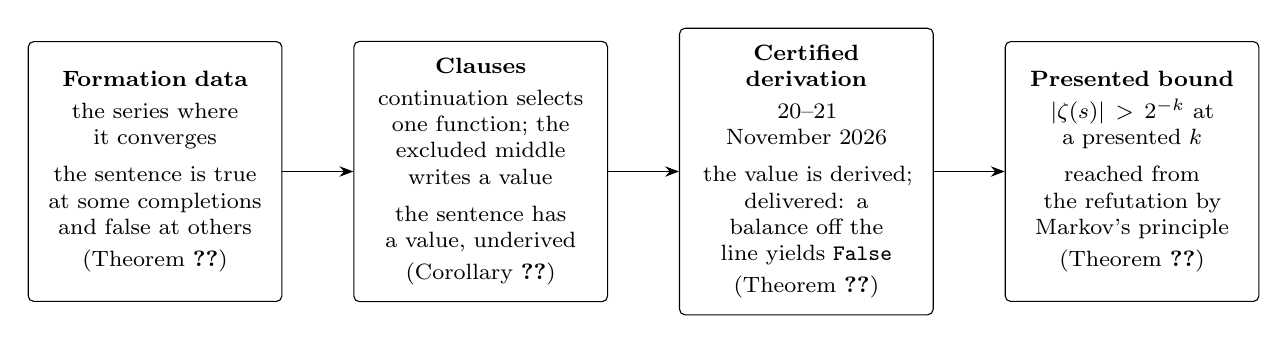
\begin{tikzpicture}[
  box/.style={draw, rounded corners=2pt, align=center, inner sep=6pt, text width=2.8cm, minimum height=3.3cm, font=\footnotesize, execute at begin node={\hyphenpenalty=10000\exhyphenpenalty=10000}},
  lab/.style={font=\scriptsize, align=center, text width=2.1cm},
  >={Stealth[length=5pt]}]
\node[box] (a) {\textbf{Formation data}\\[2pt] the series where it converges\\[4pt] the sentence is true at some completions and false at others\\[2pt] (Theorem~\ref{thm:both})};
\node[box, right=0.9cm of a] (b) {\textbf{Clauses}\\[2pt] continuation selects one function; the excluded middle writes a value\\[4pt] the sentence has a value, underived\\[2pt] (Corollary~\ref{cor:before})};
\node[box, right=0.9cm of b] (c) {\textbf{Certified derivation}\\[2pt] 20--21 November 2026\\[4pt] the value is derived; delivered: a balance off the line yields \False\\[2pt] (Theorem~\ref{thm:defence})};
\node[box, right=0.9cm of c] (d) {\textbf{Presented bound}\\[2pt] $|\zeta(s)|>2^{-k}$ at a presented $k$\\[4pt] reached from the refutation by Markov's principle\\[2pt] (Theorem~\ref{thm:markov})};
\draw[->] (a) -- (b);
\draw[->] (b) -- (c);
\draw[->] (c) -- (d);
\end{tikzpicture}
\caption{The sentence of the hypothesis at four stages. The first passage is made by clauses and was in place before the archive; the second is the content of the archive; the third is the logic's own clause.}\label{fig:stages}
\end{figure}

\paragraph{Why this matters.} Three stages are now separate, the first three of Figure~\ref{fig:stages}; the fourth is the subject of Section~\ref{sec:delivers}. On its formation data the sentence has both truth values across the completions, and no sound system of rules derives it; in the three-valued semantics of Stephen Kleene (1909--1994), in which a statement that the data leave unverified and unrefuted takes a third value, it takes that value~\citep{kleene52,tv}. With the continuation among the premises the sentence is about one function, and with the excluded middle among the rules it has a value; that value was asserted, by a derivation of one step, from the day the definition entered the library, and neither value was derived. With the certification as its sponsor, the archive derives which. The passage from the first stage to the second is in the definition of the term \lean{riemannZeta} and in the three axioms; the 17 million lines of the archive are the passage from the second stage to the third.

\section{The certified theorem as a law of the whole numbers: a sponsor stronger than the hypothesis}\label{sec:sponsor}

The author's note speaks of a proof of the hypothesis, formalized without assumptions, and the joint statement certifies that the statement and the proof are correct~\citep{alpoge,leanblog}. This section states what a derivation in the rules establishes about the whole numbers. It is the part of the note that bears on the claim, and its statements hold of every law of the whole numbers that the rules derive.

\begin{proposition}[A derived law over the whole numbers]\label{prop:tallies}
Let $Q$ be a property of whole numbers such that, at each whole number $n$ at which $Q$ holds, the rules derive $Q(n)$. Suppose that the rules derive the law ``$Q$ fails at every whole number.'' Sponsor: the rules are consistent. Then $Q$ fails at every whole number.
\end{proposition}

\begin{proof}
If $Q$ held at a whole number $n_0$, the rules would derive $Q(n_0)$, and from the law they derive the counter-inscription of $Q(n_0)$. The sponsor excludes this.
\end{proof}

The hypothesis has a form to which the proposition applies. By the criterion of Guy Robin of 1984, in the elementary form that Jeffrey Lagarias (born 1949) gave it in 2002, the hypothesis holds exactly when $\sigma(n)\le H_n+e^{H_n}\log H_n$ at every whole number $n\ge1$, where $\sigma(n)$ is the sum of the divisors of $n$ and $H_n=1+\tfrac12+\dots+\tfrac1n$~\citep{robin84,lagarias02}. The verification record reports that the archive, joined with an independent formalization of the two criteria, derives this inequality at every $n$ as a theorem that rests on the same three axioms, and that the independent checkers accept the joined proof~\citep{sutherland}. Let $Q(n)$ say that $\sigma(n)$ exceeds $H_n+e^{H_n}\log H_n$. Where $Q(n)$ holds, a computation of both sides to enough rational accuracy confirms it, and the rules replay the computation. So, on the sponsor that the rules are consistent, the inequality holds at every whole number. In the other direction, one whole number at which $Q$ held would yield, with the certified theorem, a derivation of \False{} in the rules.

\paragraph{Why this matters.} The certification is a statement about derivation: a term of the stated type exists, and the checkers accept it. It becomes a statement about the whole numbers through Proposition~\ref{prop:tallies}, and the sponsor of that proposition is a statement that the rules leave underived (Theorem~\ref{thm:second}). The sponsor is supplied from outside the rules. For the type theory of the prover's third version, Mario Carneiro derived its consistency in 2019 from the set theory of Zermelo and Fraenkel with the axiom of selection (classically, the axiom of choice) and, for each whole number $n$, the existence of $n$ inaccessible cardinals, sizes so large that the sets below each of them satisfy the axioms of the set theory~\citep{carneiro}; Lorenzo Bresolin and Marcello Mamino state in 2026 that the prover's type theory and that set theory with infinitely many inaccessible cardinals derive the same statements of second-order arithmetic, the arithmetic of the natural numbers and of sets of them~\citep{bresolinmamino}; and the joint statement reports that two of the checkers used carry a formal proof, relative to set theory, of their own soundness~\citep{leanblog}. The warrant of the certified theorem as a fact about the whole numbers is thus the consistency of that set theory, a statement of the kind that Corollary~\ref{cor:alone} describes: the completed rules assert that it has a value, and no consistent system of this kind derives its own consistency.

Throughout the rest of this section $Q(n)$ is the property that $\sigma(n)$ exceeds $H_n+e^{H_n}\log H_n$; $L$ is the law ``$Q$ fails at every whole number,'' which by the criterion of Robin and Lagarias holds exactly when the hypothesis does; $K$ is the statement that the rules are consistent; and $\mathrm{Con}$ is the statement of arithmetic of Theorem~\ref{thm:second} that expresses $K$. ``The certification'' as a sponsor includes the verification record's derivation of the law $L$ described above.

\begin{theorem}[What the certified derivation establishes outright]\label{thm:outright}
Sponsor: the certification. Then the following hold.
\begin{enumerate}[leftmargin=2em,itemsep=1pt]
\item A whole number $n_0$ at which $Q$ holds yields, by a finite construction, a derivation of \False{} in the rules.
\item Item~(1) has no further sponsor: it holds whether the rules are consistent or derive \False.
\item The existence of the certified derivation does not by itself yield the law: if the rules derive \False, they derive $L$ whether $Q$ fails at every whole number or holds at some.
\end{enumerate}
\end{theorem}

\begin{proof}
(1) Let $Q$ hold at $n_0$. The two sides of the inequality at $n_0$ are computed to a rational accuracy that separates them, and the rules replay the computation; this is a derivation of $Q(n_0)$. The derivation of $L$, followed by the rule that passes from a law to its instance at $n_0$, is a derivation of the counter-inscription of $Q(n_0)$. The two, joined by the rule that passes from a statement and its counter-inscription to \False, form a derivation of \False. Each step writes a finite tree from finite trees that are given. (2) The construction of~(1) uses the derivation of $L$ and the computation at $n_0$, and it uses nothing about the other derivations of the rules. (3) From a derivation of \False{} the rules derive every statement, since \False{} has no rule of derivation and is eliminated into any statement (Section~\ref{sec:values}); in that case the existence of a derivation of $L$ carries no information about $Q$.
\end{proof}

\begin{proposition}[The four cases]\label{prop:fourcases}
Of the four combinations
\[
L\ \text{and}\ K,\qquad L\ \text{and not}\ K,\qquad \text{not}\ L\ \text{and not}\ K,\qquad \text{not}\ L\ \text{and}\ K,
\]
Theorem~\ref{thm:outright}(1) excludes the fourth and no other. The second and the third would each be shown by one finite record whose check is a computation: a derivation of \False, and for the third also a whole number at which $Q$ holds. The first is confirmed by no finite computation.
\end{proposition}

\begin{proof}
Theorem~\ref{thm:outright}(1) is the statement ``if not $L$, then not $K$.'' A conditional fails exactly when its premise holds and its conclusion fails, which here is the fourth combination; in each of the other three the premise fails or the conclusion holds. So the statement excludes the fourth and admits the other three; in particular it admits the second, in which $L$ and ``not $K$'' both hold, so that it is not the statement that exactly one of the two holds. A derivation of \False{} is a finite tree that a finite computation checks, and a whole number at which $Q$ holds is confirmed by a finite computation; these are the records of the second and third combinations. For the first, $L$ says of every whole number $n$ that the computation at $n$ comes out one way, and $K$ says of every whole number that it does not code a derivation of \False. A finite computation confirms finitely many instances of each, and each has instances beyond every finite list. A derivation of $L$ or of $\mathrm{Con}$, in the rules or in another system, is a finite record too; what it shows, it shows on the sponsor that the system in which it stands is consistent, a statement of the same kind as $K$. The statements about the conditional are checked in the note's Lean file (\lean{excludes\_fourth\_case}, \lean{first\_three\_cases\_admitted}, \lean{conditional\_is\_not\_exclusive}).
\end{proof}

\begin{theorem}[The sponsor is a stronger statement than the law]\label{thm:stronger}
Sponsor: the certification. Then:
\begin{enumerate}[leftmargin=2em,itemsep=1pt]
\item if $K$, then $L$;
\item under the further sponsor $K$, the rules derive $L$, they leave $\mathrm{Con}$ underived, and they leave underived the statement ``if $L$, then $\mathrm{Con}$.''
\end{enumerate}
\end{theorem}

\begin{proof}
(1) is Proposition~\ref{prop:tallies}, with the certification supplying the derivation of the law. (2) The rules derive $L$ by the certification. They leave $\mathrm{Con}$ underived by Theorem~\ref{thm:second}. If they derived ``if $L$, then $\mathrm{Con}$,'' then with the derivation of $L$ and the rule that passes from a conditional and its premise to its conclusion they would derive $\mathrm{Con}$.
\end{proof}

\begin{theorem}[L\"ob, 1955]\label{thm:lob}
Write $\mathrm{Pr}(x)$ for the formula ``some $y$ has $\mathrm{Prf}(y,x)$'' of the proof of Theorem~\ref{thm:rosser}, which says that the statement with code $x$ is derived by the rules, and write $\Box A$ for $\mathrm{Pr}(\ulcorner A\urcorner)$ and $A\to B$ for ``if $A$, then $B$.'' Sponsors: the diagonal lemma, fact~(c) of that proof; and the three derivability conditions for the rules, namely (D1) if the rules derive $A$, they derive $\Box A$; (D2) the rules derive $\Box(A\to B)\to(\Box A\to\Box B)$; (D3) the rules derive $\Box A\to\Box\Box A$. Then, for every statement $A$ of arithmetic, the rules derive $\Box A\to A$ exactly when they derive $A$.
\end{theorem}

\begin{proof}
If the rules derive $A$, they derive every conditional whose conclusion is $A$, and so $\Box A\to A$. Conversely, suppose that they derive $\Box A\to A$. The diagonal lemma, applied to the formula ``if $\mathrm{Pr}(x)$, then $A$,'' gives a statement $\psi$ for which the rules derive $\psi\to(\Box\psi\to A)$ and $(\Box\psi\to A)\to\psi$. From the first of these, (D1) gives a derivation of $\Box\bigl(\psi\to(\Box\psi\to A)\bigr)$, and (D2) then gives $\Box\psi\to\Box(\Box\psi\to A)$. A second use of (D2) gives $\Box(\Box\psi\to A)\to(\Box\Box\psi\to\Box A)$. Chaining the two conditionals, the rules derive $\Box\psi\to(\Box\Box\psi\to\Box A)$. By (D3) they derive $\Box\psi\to\Box\Box\psi$, and so $\Box\psi\to\Box A$; with the supposition, $\Box\psi\to A$. By the second property of $\psi$ they derive $\psi$; by (D1), $\Box\psi$; and so $A$. The argument is that of~\citet{lob}. The derivability conditions are those of~\citet{hilbertbernays} in L\"ob's form, and~\citet{smorynski} proves them for theories of this kind. The passage from the three conditions and the fixed point to the conclusion is checked in the note's Lean file for an arbitrary system of derivation that has them (\lean{lob}, \lean{lob\_iff}).
\end{proof}

\noindent Two instances matter here. With \False{} for $A$, the statement $\Box\False\to\False$ is $\mathrm{Con}$, and the theorem says that the rules derive their own consistency exactly when they derive \False; this is Theorem~\ref{thm:second} once more. With the law $L$ for $A$, it says that the rules derive ``if the rules derive $L$, then $L$'' exactly when they derive $L$. The statement that the rules are right about this one law cannot be had from the rules as a further assurance: a derivation of it and a derivation of the law come to the same.

\begin{theorem}[The progression of sponsors; Turing, 1939]\label{thm:ladder}
Let $R_0$ be the rules, and for each whole number $n\ge0$ let $R_{n+1}$ be $R_n$ with the statement $\mathrm{Con}(R_n)$, ``no number codes a derivation of \False{} in $R_n$,'' added as an axiom. Sponsors: each $R_n$ is consistent, and Theorem~\ref{thm:second} holds of each. Then:
\begin{enumerate}[leftmargin=2em,itemsep=1pt]
\item $R_{n+1}$ derives $\mathrm{Con}(R_n)$, and $R_n$ does not;
\item if $R_n$ derives a law ``$Q'$ fails at every whole number,'' for a property $Q'$ such that $R_n$ derives $Q'(m)$ at each whole number $m$ at which it holds, then the law holds on the sponsor that $R_n$ is consistent, a statement that $R_{n+1}$ derives and $R_n$ does not;
\item for no $N$ does $R_N$ derive $\mathrm{Con}(R_n)$ for every $n$.
\end{enumerate}
\end{theorem}

\begin{proof}
(1) $\mathrm{Con}(R_n)$ is an axiom of $R_{n+1}$. The system $R_n$ consists of the rules and finitely many further axioms, so its derivations are checked by computation and it contains arithmetic; by the second sponsor it leaves $\mathrm{Con}(R_n)$ underived. (2) Proposition~\ref{prop:tallies} holds with $R_n$ in the place of the rules, by the same proof; (1) gives the rest. (3) If $R_N$ derived $\mathrm{Con}(R_n)$ for every $n$, it would derive $\mathrm{Con}(R_N)$, against~(1).
\end{proof}

\noindent The progression is that of Alan Turing (1912--1954), who studied in 1939 the systems obtained from a given one by adding, step after step, the statement of its consistency~\citep{turing39}. In the book of the present author and Ryan J. Buchanan it is the reflection ladder: an attempt to certify, inside one system, that what the system derives holds at every stage leads to a principle of reflection, which that system leaves underived, and from there to an ascent through stronger systems that no step closes; and by the theorem of Henry Gordon Rice (1920--2003) of 1953 no computation decides, from the code of a procedure, whether the procedure yields a valid certificate at every stage~\citep{metatheory,rice53}.

\begin{proposition}[What the checks test, and what the words of the announcement cover]\label{prop:checks}
\leavevmode
\begin{enumerate}[leftmargin=2em,itemsep=1pt]
\item The joint statement reports four checks~\citep{leanblog}: that the statement is the library's \lean{RiemannHypothesis}, which experts reviewed; that the archive compiles, and that many people obtained the same exported proof; that a separately written statement matches the theorem proved, by two comparison tools; and that the prover's kernel and several independently written checkers accept the exported proof. The first is a reading. The other three are finite computations on the archive and on the exported proof.
\item None of the four is a derivation of $\mathrm{Con}$, and none tests it: each concerns one term. Under the sponsor $K$, no check that is carried out as a derivation in the rules establishes $\mathrm{Con}$ (Theorem~\ref{thm:second}).
\item The joint statement adds that two of the checkers carry a formal proof, relative to set theory, that they accept no false proof. That proof concerns the programs, and its own sponsor is the consistency of the set theory to which it is relative.
\item The author's note describes the formalized argument with the words ``without assumptions''~\citep{alpoge}. It does not name the three axioms, and it says nothing of the consistency of the rules or of what a check leaves untested. In the usage of the prover's community such words describe a derivation with no unproved hypothesis and no axiom beyond the three.
\end{enumerate}
\end{proposition}

\begin{proof}
Items~(1), (3) and~(4) are read from the two documents. Item~(2) follows from item~(1) and Theorem~\ref{thm:second}.
\end{proof}

\paragraph{Why this matters.} These statements are the note's criticism of the claim, and they are bounded as follows. The derivation is not what is criticized: with the certification as its sponsor it exists. What is criticized is the passage from ``derived'' to ``proved of the whole numbers,'' to ``without assumptions,'' and to ``correct'' as a word for more than the term. A derivation in the rules establishes outright that the law holds or the rules derive \False, and the certificate contains no means of telling which (Proposition~\ref{prop:fourcases}). The favourable case is held on evidence: the set theory of Zermelo and Fraenkel has been in use for a century, and its extension by inaccessible cardinals for some sixty years, and no derivation of \False{} has come to light in either. That is evidence, and it is not a derivation. No derivation of it can stand in the rules (Theorem~\ref{thm:second}), a derivation of it elsewhere needs the next sponsor (Theorem~\ref{thm:ladder}), and the rules cannot even vouch for themselves about the one law in question beyond deriving it (Theorem~\ref{thm:lob}). The sponsor is, moreover, a stronger statement than the one it sponsors (Theorem~\ref{thm:stronger}). Written with its sponsor, the claim reads: the law of the hypothesis holds, on a premise that implies the hypothesis and is not implied by it. Every law of the whole numbers that the rules derive stands in this way, and the note does not single out the archive; the usage of mathematics leaves the sponsor unsaid. The present case differs in what has been said of it. The words ``without assumptions'' are accurate of hypotheses and silent about the sponsor; the word ``correct'' is accurate of the term and silent about the sponsor; and a reader who takes either for the statement that the hypothesis holds of the whole numbers has taken a derivation for the truth of its sponsor.

\begin{proposition}[The rules reach beyond the set theory in arithmetic]\label{prop:beyond}
Write $\mathsf{ZFC}$ for the set theory of Zermelo and Fraenkel with the axiom of selection. Sponsors: $\mathsf{ZFC}$ is consistent; and the statement of~\citet{bresolinmamino} that the prover's type theory with its axioms and $\mathsf{ZFC}$ with infinitely many inaccessible cardinals derive the same statements of second-order arithmetic. Then the rules derive a statement of arithmetic that $\mathsf{ZFC}$ leaves underived: the statement that $\mathsf{ZFC}$ is consistent. Consequently a derivation of a statement of arithmetic in the rules is not thereby a derivation of it in $\mathsf{ZFC}$.
\end{proposition}

\begin{proof}
If $\kappa$ is an inaccessible cardinal, the collection of the sets of rank below $\kappa$ satisfies every axiom of $\mathsf{ZFC}$~\citep[ch.~12]{jech}. So $\mathsf{ZFC}$ with one inaccessible cardinal derives that $\mathsf{ZFC}$ has a model, and with it the statement of arithmetic $\mathrm{Con}(\mathsf{ZFC})$ that no number codes a derivation of \False{} from the axioms of $\mathsf{ZFC}$, since a theory with a model derives no falsehood. By the second sponsor the rules derive $\mathrm{Con}(\mathsf{ZFC})$. By the second incompleteness theorem and the first sponsor, $\mathsf{ZFC}$ does not.
\end{proof}

\paragraph{Why this matters.} What was certified is a derivation in the prover's rules. Whether the sentence of the hypothesis has a derivation in $\mathsf{ZFC}$, the theory to which the word ``proved'' ordinarily refers in mathematics, is a further question, and the certification leaves it where it was: the proposition shows that derivability in the rules does not settle it in general. For the truth of the law over the whole numbers the sponsor is the consistency of the rules (Proposition~\ref{prop:tallies}), which is a stronger statement than the consistency of $\mathsf{ZFC}$.

\begin{theorem}[The certified derivation does not prove the hypothesis]\label{thm:notproof}
Sponsor: the certification. The certified derivation is a derivation of the sentence of the hypothesis in the prover's rules, and it is not a proof of the hypothesis in any of the following three senses.
\begin{enumerate}[leftmargin=2em,itemsep=1pt]
\item \emph{Of the whole numbers.} It does not establish outright that the law $L$ holds. It establishes that $L$ holds if the rules are consistent. That premise implies $L$ and is not implied by it in the rules; the rules leave it underived if it holds; and a derivation of it in another system establishes it on the sponsor that the other system is consistent.
\item \emph{From the series.} It is not a derivation from the data that form the sentence, the zeta series on the half-plane where it converges with the class of its completions and the form of the sentence. Those data give the sentence both truth values.
\item \emph{In the set theory.} Under the sponsors of Proposition~\ref{prop:beyond}, the rules derive a statement of arithmetic that $\mathsf{ZFC}$ leaves underived. A derivation in the rules is therefore not thereby a derivation in $\mathsf{ZFC}$, and none of the four checks of the certification concerns a derivation in $\mathsf{ZFC}$.
\end{enumerate}
\end{theorem}

\begin{proof}
(1) The first sentence is Theorem~\ref{thm:outright}(3), and the second is Proposition~\ref{prop:tallies}. Of the third, the first clause is Theorem~\ref{thm:stronger}, the second is Theorem~\ref{thm:second}, and the last is Theorem~\ref{thm:ladder}(2), since the statement that a system is consistent is itself a law of the form to which that item applies: no whole number codes a derivation of \False. (2) Theorem~\ref{thm:both} and Corollary~\ref{cor:notfrom}. (3) Proposition~\ref{prop:beyond} and Proposition~\ref{prop:checks}(1).
\end{proof}

\noindent The first sense is not particular to the hypothesis. No derivation in the rules proves a law of the whole numbers in that sense, since the argument is the same for each; in that sense every theorem of the library that states such a law stands as the certified theorem does, on the consistency of the rules. The second and the third senses are particular: the second to a sentence that is formed by a series and speaks of values that a continuation writes, the third to rules that reach beyond the set theory in arithmetic. What the certified derivation is, with the certification as its sponsor, is a derivation. The sentence ``the Riemann hypothesis has been proved'' is true of it in the sense in which ``proved'' means ``derived in the prover's rules,'' and in no sense that says more.



\section{What the certified derivation delivers}\label{sec:delivers}

\begin{theorem}[The refutation of a balance, and the defence]\label{thm:defence}
\leavevmode
\begin{enumerate}[leftmargin=2em,itemsep=1pt]
\item The statement \lean{EveryCharacter}, and the hypothesis that the step \lean{rh\_of\_right} receives, conclude that a value is apart from ``0.'' By the prover's definitions this conclusion is the statement that the equation of the value with ``0'' yields \False.
\item Sponsor: the certification. At every point $s$ of the critical strip off the critical line there is a complex number $b$ with $\zeta(s)\cdot b=1$. Conversely, this statement yields the certified theorem.
\end{enumerate}
\end{theorem}

\begin{proof}
(1) The two statements are printed in Part~2a of the Supporting Information. ``Apart from'' unfolds to the counter-inscription of an equation, and the counter-inscription of a statement to ``the statement yields \False,'' by the prover's definitions (Section~\ref{sec:values}; the declarations \lean{apart\_unfolds} and \lean{counter\_inscription\_unfolds}).

(2) Let $s$ lie in the strip off the critical line. Suppose $\zeta(s)$ is ``0.'' The point $s$ is apart from every $-2(n+1)$ and from $1$, these lying outside the strip, so the certified theorem places $s$ on the critical line, where it does not lie. So the equation of $\zeta(s)$ with ``0'' yields \False: $\zeta(s)$ is apart from ``0.'' In a field a value apart from ``0'' has an inverse; this is the guarded clause of the library's class of fields, which reads ``for $a$ apart from `0,' $a\cdot a^{-1}=1$'' (\lean{GroupWithZero.mul\_inv\_cancel}). Take $b=\zeta(s)^{-1}$.

Conversely, let $\zeta$ have an inverse at every point of the strip off the critical line, and let $s$ be a balance point of $\zeta$ apart from every $-2(n+1)$ and from $1$. By the proof of Theorem~\ref{thm:selection}(3), $s$ lies in the strip. If $s$ lay off the critical line, some $b$ would have $\zeta(s)\cdot b=1$, while $\zeta(s)\cdot b$ is the product of ``0'' with $b$, which is ``0'' and is apart from $1$. So it is refuted that $\re s$ is apart from $\tfrac12$, and by the excluded middle $\re s=\tfrac12$.
\end{proof}

\noindent The artifact of~\citet{tv} checks the equivalence of part~(2) against the library, as the declaration \lean{riemannHypothesis\_iff\_zeta\_inverse}.

\paragraph{Why this matters.} Part~(2) says what the certified theorem establishes with the unit in the place of the constant: the selected function has an inverse at every point of the strip off the critical line. The library shows why the positive sentence has to be said in this form. Its term $\zeta(s)^{-1}$ has a value at every $s$, completed at the balance points by the clause that the inverse of ``0'' is ``0''; ``the inverse is defined'' therefore has to be said by naming what is present, a number $b$ with $\zeta(s)\cdot b=1$. Part~(1) says in what form the archive delivers it. The product of 17 million lines is a refutation: a balance to the right of the critical line yields \False.

\begin{theorem}[Refutation, presented bound, and Markov's principle]\label{thm:markov}
Write $|z|$ for the modulus of a complex number $z$, its distance from ``0.'' Call a complex number $x$ \emph{presented by a rule} when a rule issues, at each tally $k=1,2,3,\dots$, a complex number $q_k$ with rational coordinates such that $|x-q_k|\le 2^{-k}$. A \emph{decision} on the tallies is a rule that, at each tally, succeeds or fails by a finite computation. For an $x$ presented by a rule, let the decision $d_x$ succeed at the tally $k$ when $|q_k|>2\cdot2^{-k}$, a comparison of rational numbers, and fail there otherwise.
\begin{enumerate}[leftmargin=2em,itemsep=1pt]
\item $x$ balances (classically, $x=0$) exactly when $d_x$ fails at every tally.
\item If $d_x$ succeeds at the tally $k$, then $|x|>2^{-k}$: the tally presents a bound.
\item A refutation of the balance of $x$ is therefore a refutation of ``$d_x$ fails at every tally,'' and the passage from it to a tally at which $d_x$ succeeds is an instance of the principle of Andrei Markov (1903--1979): for every decision $d$ on the tallies, if it is refuted that $d$ fails at every tally, then $d$ succeeds at some tally~\citep{markov}.
\item Conversely, if for every number presented by a rule the refutation of its balance yields a tally at which its decision succeeds, then Markov's principle holds.
\end{enumerate}
\end{theorem}

\begin{proof}
(1) If $x$ balances, then $|q_k|\le2^{-k}$ at every tally, which is below $2\cdot2^{-k}$, so $d_x$ fails at every tally. If $d_x$ fails at every tally, then $|x|\le|x-q_k|+|q_k|\le3\cdot2^{-k}$ at every tally $k$, and a modulus that lies below $3\cdot2^{-k}$ for every $k$ is ``0.''

(2) If $|q_k|>2\cdot2^{-k}$, then $|x|\ge|q_k|-|x-q_k|>2\cdot2^{-k}-2^{-k}=2^{-k}$.

(3) By~(1), ``$x$ balances'' and ``$d_x$ fails at every tally'' each yield the other, so a refutation of the first is a refutation of the second. Whether $d_x$ succeeds at a tally is settled by a comparison of rational numbers, so $d_x$ is a decision on the tallies, and the passage in question is Markov's principle at $d_x$.

(4) Let $d$ be a decision on the tallies. Let the rule issue at the tally $k$ the number $q_k=2^{-m}$ when $d$ succeeds at some tally up to $k$ and $m$ is the first such tally, and the number ``0'' when $d$ fails at every tally up to $k$. For tallies $j<k$ the numbers $q_j$ and $q_k$ agree unless $d$ first succeeds at a tally $m$ with $j<m\le k$, and then they differ by $2^{-m}$, which is at most $2^{-(j+1)}$. So the $q_k$ converge to a real number $x$ with $|x-q_k|\le2^{-k}$ at every tally, and the rule presents $x$. If $x$ balances, then $d$ fails at every tally: were $d$ to succeed at a tally, with first such tally $m$, every $q_k$ from $k=m$ on would be $2^{-m}$ and $x$ would be $2^{-m}$. So a refutation of ``$d$ fails at every tally'' is a refutation of the balance of $x$. By the hypothesis of~(4) some tally $k$ has $|q_k|>2\cdot2^{-k}$. Then $q_k$ is apart from ``0,'' so $d$ succeeds at some tally up to $k$, which is found by testing $d$ at the tallies $1,\dots,k$ in turn.
\end{proof}

\paragraph{Why this matters.} At a point $s$ of the strip with rational coordinates the value $\zeta(s)$ is presented by a rule: the summation formula of Euler and Colin Maclaurin (1698--1746) computes it to any presented accuracy~\citep[ch.~6]{edwards}. What the certified derivation delivers there, off the critical line, is the refutation of a balance (Theorem~\ref{thm:defence}). A presented bound, a tally $k$ with $|\zeta(s)|>2^{-k}$, is the result of a search, and what carries the refutation to the result of the search is Markov's principle. Part~(4) shows that this is no peculiarity of the zeta function: the passage, asked of every presented number, is the principle itself. In the terms of~\citet{tv}, Markov's principle is the logic's own completion by clause: where the data supply the refutation of a balance, the principle issues the presented magnitude that the data withheld. Over a closed rectangle of the strip, in place of a point, the pointwise bounds are gathered into one by compactness, the property that finitely many of any discs that cover the rectangle already cover it; its constructive form is the fan theorem of Luitzen Egbertus Jan Brouwer (1881--1966)~\citep{dummett}.

\begin{remark}[The passage in the prover, and a second route]\label{rem:routes}
In the prover the passage divides into two parts, each of which the note's Lean file checks. The first part leads from the refutation of ``$d$ fails at every number'' to the statement ``$d$ succeeds at some number.'' It is derived in the rules, by the excluded middle, and the prover reports that it rests on the three axioms (the declaration \lean{markov\_in\_completed\_rules}). The second part leads from that statement to a number. It is a search that tests $d$ at each number in turn, and it is defined with no axiom (the declaration \lean{present}); the prover compiles it to a program. The composite runs: for the decision that succeeds at the number $7$ and nowhere else it returns $7$ (the declaration \lean{presentFromRefutation}). Its definition rests on the three axioms, which enter in the first part alone. The search halts when a number at which $d$ succeeds exists; what the derivation supplies is the statement that one exists, and it supplies it by the clause.

There is a second route from a classical derivation to presented numbers. Harvey Friedman (born 1948) showed in 1978 that classical and intuitionistic arithmetic, and likewise the classical and the intuitionistic set theory of Zermelo and Fraenkel, derive the halting of the same programs: a derivation in the classical theory that a search halts at every input is transformed into a derivation in the theory without the excluded middle, which presents its numbers~\citep{friedman78}. The transformation takes a whole derivation as its input. A transformation of this kind for the certified derivation would be a further construction on the archive, carried through the set theory in which the prover's rules are interpreted, and its result would present the bounds with the excluded middle no longer among the premises. What was certified is the derivation in the completed rules.
\end{remark}

\section{What the certification checks, and what the certified term draws on}\label{sec:warrant}

Section~\ref{sec:sponsor} has stated on which sponsor the certified theorem is a law of the whole numbers. This section turns to the certification itself: which programs have accepted which form of the term, what the text of the sources excludes, and what the certified term draws on in the part of the archive where the hypothesis is decided.

\begin{proposition}[The state of the certification on 22 and 23 November 2026]\label{prop:state}
The verification record~\citep{sutherland} carries in its header the date 22 November 2026, 02:25 UTC, and its latest entry is timed 04:16 UTC on that day; it was read at 14:37 UTC. The notes of the checkers' repository~\citep{leannotes} were read at the same hour. The record was read again on 23 November 2026 at 01:15 UTC; its header and its latest entry were unchanged, and the runs listed below as unfinished were still listed so. The two documents report the following.
\begin{enumerate}[leftmargin=2em,itemsep=1pt]
\item \emph{Accepted.} All 175{,}187 modules compile under version~4.33.1 of the prover. A replay of every compiled module through the prover's kernel accepts all of them, and so does a replay through the independently written checker lean4lean, five modules passing after its limit on steps of computation was raised. The independently written checkers nanoda, con-leche and con-ron, the last two built from their current sources, accept the exported proof, which has 1{,}468{,}418 declarations. The five theorems rest on the three axioms. The comparison of the proved statements with a separately written statement of them, and the check of the axioms, have passed. The compiled files of the library agree byte for byte with those of the library's official build. A second build of the archive, made inside an enclosure, yields an exported proof identical to the published one, and compiled files identical to the published ones for 175{,}186 of the 175{,}187 modules; the compiled file of the remaining module has the same size and comes out with one of two contents from one compilation to the next, and the record gives no cause for this.
\item \emph{Unfinished.} Two runs are listed as running, with no result: the run of the prover's own kernel, in its default and its paranoid mode, on the exported proof as a whole; and the run of the comparison tool from end to end, whose first stages are the comparison and the check of axioms just named. The run of the comparison tool on the archive joined with the formalization of the criterion of Robin and Lagarias, which is described after Proposition~\ref{prop:tallies}, is listed in the same state. The notes of the checkers' repository say that its own build is in progress, and they record no result.
\item \emph{Declined.} The checkers con-leche and con-ron, in the versions distributed with version~4.36.0 of the prover, stop on the exported proof: they do not support a block of mutually defined inductive types of which one is reflexive, and the archive contains such a block.
\item \emph{What a pass is said to show.} The record says that a passing check shows the statements to follow from the three axioms ``according to the kernels used,'' and that it relies on those kernels and on the library's definitions. The notes add that the kernel of version~4.33.1, under which the archive is compiled, lacks corrections made in later versions, two of them for errors that, by the release notes, could be turned into a derivation of \False; that a pass by that kernel alone therefore counts as ``limited evidence''; and that a passing run still trusts the checkers, the library's definitions and its official build, the program that exports the proof, and the enclosures in which the checkers run.
\end{enumerate}
\end{proposition}

\begin{proof}
Each item is read from the two documents as they stood at the times named.
\end{proof}

\paragraph{Why this matters.} The certification is a statement that programs have accepted a term. The proposition records which programs, on which form of the term, and what was still running one day after the joint statement. The joint statement reports that the prover's kernel and the other checkers were run on the exported proof~\citep{leanblog}; in the independent record the corresponding run of the kernel was unfinished at the time of reading, while its replay of the compiled modules had passed. Several checkers written independently of one another accept the same exported proof, which makes an error shared by all of them improbable. It does not make the certified theorem independent of programs, and the record says as much in its own words.

\begin{proposition}[What the text of the sources excludes]\label{prop:scan}
In the 175{,}187 Lean files of the archive, as counts of text, the following hold.
\begin{enumerate}[leftmargin=2em,itemsep=1pt]
\item No file contains the word \lean{sorry}, \lean{admit}, \lean{axiom}, \lean{native\_decide}, \lean{unsafe}, \lean{opaque} or \lean{implemented\_by}, or the string \lean{@[extern}, \lean{ofReduceBool} or \lean{trustCompiler}.
\item The files set 33 distinct options with the command \lean{set\_option}. The name of the option \lean{debug.skipKernelTC}, which suspends the kernel's check of a declaration, occurs in no file.
\item No line declares a constant named \lean{RiemannHypothesis}, \lean{riemannZeta}, \lean{hurwitzZetaEven}, \lean{completedHurwitzZetaEven} or \lean{Gamma$\mathbb R$}, the names with which the certified sentence is written.
\item No theorem is stated as \False{} with no hypothesis.
\item Five files run a command while the archive is compiled. Each has three lines and adds one name to the list of names that the prover's aid for suggesting library lemmas leaves aside.
\item The manifest requires the library from its public repository at the pinned commit.
\end{enumerate}
\end{proposition}

\begin{proof}
Part~1 of the Supporting Information: the table of words and strings, the table of options, the two searches for declarations, and the five files with the command they run.
\end{proof}

\paragraph{Why this matters.} A scan of text is not a check of a derivation, and the proposition is offered as what it is. The sources contain none of the means by which a compiled archive can assert more than its kernel has checked, and no second definition of the words of the certified sentence. With the record's comparison of the compiled library, byte for byte, with the official build (Proposition~\ref{prop:state}(1)), items~(3) and~(6) leave the sentence that was certified as the library's sentence, which Theorem~\ref{thm:selection} identifies as the raw sentence at the continuation.

\begin{proposition}[The bound on windows: what is announced, what the route shows, and the accounts of it]\label{prop:bound}
\leavevmode
\begin{enumerate}[leftmargin=2em,itemsep=1pt]
\item \emph{Announced.} The note of the archive's author describes the argument for the bound as a chain of theta lifts between unitary groups, of length about $\sqrt X$ for a sum over the prime powers up to $X$, with a lower bound for the divisibility of the lifted quantities and with the slope inequality of Jean-Beno\^it Bost (born 1961), an inequality of the geometry of lattices over number fields that holds for an injective map between them~\citep{alpoge,bost96,riemannrev}.
\item \emph{On the route.} The archive defines a type \lean{GeoP} of conditions on its objects, and three terms of that type. The term \lean{geoOf} asks for a witness: a whole number $c>0$ with a property that the archive names \lean{IsGeoOf}, and a second property that it names \lean{HasTrueSurf}. The term \lean{anyGeometry} is defined to hold of every object. The closure \lean{geoCl} of a condition holds wherever the condition holds, so \lean{geoCl anyGeometry} holds of every object. A condition $\Gamma$ of the type enters the objects of this part of the archive as follows. The parameters of a family carry a condition, set by the third argument of their constructor \lean{parametersOfExtension}; from it the archive forms a component \lean{OX}; and the record \lean{OAt} of that component has a field \lean{geo}, which is a derivation of $\Gamma$ at the object. The lemmas of this part are stated for a variable $\Gamma$; of the 291 places of that constructor, 240 pass the variable. Where the text passes a condition by name, the name is \lean{anyGeometry}. That name stands at 162 places in 24 files: at 151 of them inside \lean{geoCl anyGeometry}, at 4 inside the component or its record, at 6 as the last argument of a lemma, and once in its own definition. The term \lean{geoOf} stands at 4 places in 2 files: the file that defines it, and one file of three lemmas about it, in which it is applied to a variable. Of the three lemmas, one is named a second time in that file, and none is named in any other file of the archive. (Two further declarations, of other types, carry the same short name; the word \lean{geoOf} occurs at 16 places in 10 files.) On the route (Proposition~\ref{prop:chain}(6)), the theorem \lean{hypotheses\_nonempty\_of\_unramified\_exponents\_alt} concludes that the bundle \lean{HypsAlt} has a member. Two of its premises are stated for \lean{geoCl anyGeometry}: one for a condition that the archive names \lean{FunctionalCondition}, the other for one that it names \lean{CovolumeBoundThirdPlaceSeries}. The theorem \lean{nonempty\_hyps\_definite\_side\_of\_closed\_bound} supplies them and writes \lean{geoCl anyGeometry} at three places.
\item \emph{Accounts.} The author's note says of the part of the argument on automorphic forms that he has ``little mastery'' of it and that he paraphrases a summary made by the language model; it presents the Lean files in the place of a written proof, and it mentions more than 250{,}000 pages of generated text~\citep{alpoge}. The note of~\citet{zhang} describes the announced argument; it says that its account, from the second section on, was drafted with a language model that read the Lean files and was then rewritten by its author, and that the author does not vouch that the account matches the Lean files. The guide of~\citet{riemannrev} reads this part from the Lean source and the announcement and does not derive it again. An unsigned schematic account names as unverified the step by which repeated theta lifts yield divisibility while the sizes stay under control~\citep{schematic}.
\end{enumerate}
\end{proposition}

\begin{proof}
(1) and (3) are read from the documents cited. (2) Part~2e of the Supporting Information prints the definitions named, with the rule \lean{base} of the closure, which derives the closure of a condition at an object from the condition at that object. It lists the declarations whose stated type is \lean{GeoP}, the declarations that carry the short name \lean{geoOf} with the places of each, and the lemmas about the term \lean{geoOf} with the places at which each is named. It tallies the argument that follows \lean{geoCl}, the places of \lean{anyGeometry}, and the condition passed at each place of \lean{parametersOfExtension}, of the component \lean{OX} and of its record \lean{OAt}. And it counts the places of \lean{geoCl anyGeometry} in the statement of the first theorem, with the conditions that its two premises carry, and in the text of the second.
\end{proof}

\paragraph{Why this matters.} The three parts do not meet. What is announced for the bound is an argument in which an inequality of geometry is applied to objects built by theta lifts. What the text of the archive shows is that its lemmas of this part take a condition $\Gamma$ on their objects as a variable, and that the condition which the text puts in the place of that variable, outside one lemma that no other declaration names, is the condition that every object satisfies. The certified theorem has no variable left in it, so on the way to the final theorem every $\Gamma$ has been filled; and the condition that asks for a geometric witness is defined, has three lemmas, and is named by no declaration outside the file of those lemmas. As far as the names in the text reach, the certified term therefore draws nothing from a condition of this type: where its objects carry the field \lean{geo}, every object fills it. Of the four accounts of the argument, none is offered by its author as a derivation of the bound that the author has checked. The author of the archive writes that his command of the part on automorphic forms is slight, and he presents the Lean files in the place of a written proof; the note of Zhang was drafted with a language model that read those files, and its author does not vouch that it matches them. For the bound on windows, which is the part in which the hypothesis is decided, the warrant of the certified theorem on 22 November 2026 is therefore the check of Proposition~\ref{prop:state}.

\begin{proposition}[The geometric condition in the exported proof]\label{prop:compiled}
The following are facts about the published list of the names in the exported proof (Section~\ref{sec:method}).
\begin{enumerate}[leftmargin=2em,itemsep=1pt]\sloppy
\item \emph{The condition that every object satisfies is in the exported proof.} The list holds \lean{GlobalTheory.Mem.Top.Bl.anyGeometry} and the closure \lean{geoCl} of the same namespace, the constructor \lean{parametersOfExtension}, and the two theorems of Proposition~\ref{prop:bound}(2).
\item \emph{The condition that asks for a geometric witness is not.} No line of the list ends in the name \lean{geoOf}, \lean{IsGeoOf} or \lean{HasTrueSurf}.
\item \emph{A divisor record is filled from a degenerate model.} The list holds \lean{geoDegenerate}, \lean{divXFl}, \lean{geoOver\_stages} and \lean{divEx\_prov}. The first is a term of the archive's type \lean{DV.Geo} of geometries in which the varieties are the natural numbers, the function field of each is the base field, every divisor is effective, every space of sections is the whole field, and the conditions that the type names \lean{nef}, \lean{big} and \lean{bpf} are defined to hold of every object. The second is the divisor record obtained from a given one by putting that term in the place of its geometry. The third states, of every divisor record, a condition \lean{GeoOver} whose condition on levels is the one that holds of every level, and its proof supplies \lean{divXFl}. The fourth derives the existence of the divisor data under the hypothesis that the place for conditions holds \lean{OX anyGeometry}.
\item \emph{The declarations that tie a divisor record to a family are not in the exported proof.} No line of the list ends in the name \lean{GeoTied}, \lean{GeoTiedM}, \lean{FormsTieX}, \lean{formsTieX\_of\_cusp}, \lean{MumfordU}, \lean{CurveHTDom}, \lean{chern\_linRoot\_pow} or \lean{shimura\_sheaf\_of\_indefinite\_subspace}. In the archive \lean{GeoTied} is the statement that a divisor record is tied to a family over its geometry, and \lean{FormsTieX} the statement that the sections which the record assigns to lattice vectors lie in the span of the forms of the family.
\item \emph{Declarations named for arithmetic geometry stand elsewhere in the exported proof.} The list holds, among others, \lean{ArithHilbertSamuel}, \lean{KawamataViehweg}, \lean{hodge\_bundle\_isNef\_isBig\_of\_weight}, \lean{chowla\_selberg\_eta} and \lean{topCovolG\_alt\_alt}. The note has read the statement of the first, which speaks of Hermitian line bundles over schemes of the library, and the names of the others; it has not read their derivations.
\end{enumerate}
\end{proposition}

\begin{proof}
Part~7 of the Supporting Information looks up each name in the list and prints the lines found; it prints the definition of \lean{geoDegenerate} field by field, the opening of the definition of \lean{divXFl}, and the statements of \lean{geoOver\_stages}, \lean{divEx\_prov}, \lean{GeoTied} and \lean{FormsTieX}.
\end{proof}

\paragraph{Why this matters.} Proposition~\ref{prop:bound}(2) was a statement about the text of the archive, and it left open what the compiled term contains. The list of the exported proof closes that gap in both directions. The condition that every object satisfies is in the exported proof, and with it a model of the archive's geometries in which the geometric conditions hold by definition; the condition that asks for a geometric witness, and the declarations by which a divisor record would be tied to a family over a variety, are not. At this layer the certified term is therefore other than the argument that was announced: where the announcement speaks of an inequality of geometry applied to objects built by theta lifts, the exported proof carries, on the side of the divisor record, a condition and a model that every object satisfies. The statement is confined to this layer. Declarations that the archive names for arithmetic geometry stand elsewhere in the exported proof (item~5), and the note makes no statement about what they contribute.

\begin{remark}[On the inference that nothing is proved]\label{rem:nothing}
\citet{nielsen} reported the definition of \lean{anyGeometry} and concluded that the proposed proof is invalid; in the words of her abstract, the code compiles but ``nothing is proved.'' A later check of the report found the definition in 24 files and left open whether the final theorem depends on it~\citep{chu}. Proposition~\ref{prop:bound}(2) settles that point for the text: the route passes through the definition. Proposition~\ref{prop:compiled} settles it for the exported proof: the definition is one of its declarations. The conclusion, however, does not follow from the observation. A definition is an abbreviation: when the rules derive a statement in which a defined name does not occur, they derive it also with every occurrence of the name in the derivation replaced by the term that defines it. The library's statement \lean{RiemannHypothesis} does not contain the name \lean{anyGeometry}. So, with the certification as sponsor, the rules derive the certified sentence from the three axioms by a derivation in which the condition that holds of every object stands, written out, at those places; that the condition has a name adds nothing to what is derived and takes nothing from it. Nor can a condition that holds of every object stand in for an unproved assumption: a theorem stated for it is stated for every object, and the kernel checks its derivation as it checks every other. The archive does not conceal conditions of this kind either. A scan of its text finds 17 definitions whose whole body is the statement \True{} or a function with the value \True{} at every argument (Supporting Information, Part~1). The condition \lean{anyGeometry} is one of them, and the others carry names such as \lean{trivialClassCondition}, \lean{noCondition}, \lean{TrivialCondition} and \lean{UnusedSlot55}: the general lemmas of the archive have places for conditions, and at some of those places the condition supplied is the one that every object satisfies. What the observation does show is the content of Proposition~\ref{prop:bound}(2): the certified term draws nothing from a condition of the type \lean{GeoP}. The certification is a certification of that term and of the sentence it derives. That the term carries out the announced argument is a further statement, which the certification does not make and which none of the accounts cited establishes.
\end{remark}


\section{Position}\label{sec:position}

The note takes the following position, bounded to what its statements establish.

\begin{enumerate}[leftmargin=2em,itemsep=4pt]
\item \textbf{The certified derivation does not prove the Riemann hypothesis.} It derives the sentence of the hypothesis in the prover's rules. With the certification as its sponsor that derivation exists, and the note does not dispute it. It is not a proof of the hypothesis in three senses (Theorem~\ref{thm:notproof}): it does not establish outright that the hypothesis holds of the whole numbers; it is not a derivation from the zeta series; and it is not a certified derivation in the set theory to which the word ``proved'' ordinarily refers. The author's note states the belief that the hypothesis is proved and describes the formalized argument with the words ``without assumptions''; the joint statement certifies that the statement and the proof are correct. Those words cover the derivation.

\item \textbf{What the derivation establishes outright.} Outright, the derivation establishes that a whole number at which the law of the hypothesis failed would yield a derivation of \False{} in the rules, and no more than that about the whole numbers (Theorem~\ref{thm:outright}). Of the four combinations of ``the law holds'' and ``the rules are consistent'' it excludes one, and it holds no means of telling which of the other three is the case (Proposition~\ref{prop:fourcases}).

\item \textbf{The sponsor is a stronger statement than the hypothesis.} The law holds on the sponsor that the rules are consistent (Proposition~\ref{prop:tallies}). That sponsor implies the hypothesis and is not implied by it in the rules (Theorem~\ref{thm:stronger}); the rules, if consistent, leave it underived (Theorem~\ref{thm:second}); they derive that they are right about this one law exactly when they derive the law (Theorem~\ref{thm:lob}); and a derivation of the sponsor in a stronger system rests on the consistency of that system, at each step of a progression that no step closes (Theorem~\ref{thm:ladder}). A proof of the hypothesis as a law of the whole numbers, in the sense that the word carries when the sponsor is left unsaid, would have to supply the sponsor, and to establish the sponsor is to establish more than the hypothesis.

\item \textbf{What is held, and on what.} The favourable case, in which the law holds and the rules are consistent, is the one that no finite computation confirms: each of its halves is a law over all the whole numbers. Each of the other cases would be shown by one finite record, a whole number at which Lagarias's inequality fails or a derivation of \False. No such record has come to light in the century during which the set theory of Zermelo and Fraenkel has been in use, nor in the sixty years of its extension by inaccessible cardinals, on which the rules rest. That is the evidence on which the favourable case is held. It is evidence, and it is not a derivation.

\item \textbf{What the checks test.} The four checks of the certification are a reading and three finite computations about one term. None of them tests the sponsor, and none could establish it by a derivation in the rules (Proposition~\ref{prop:checks}). The words ``without assumptions'' are accurate of unproved hypotheses and of axioms beyond the three; they are silent about the sponsor, of which the author's note says nothing. On 23 November 2026 the public record of the checks still listed two runs as unfinished, among them the run of the prover's own kernel on the exported proof as a whole (Proposition~\ref{prop:state}).

\item \textbf{This is the standing of every law that the rules derive.} The note does not single out the archive. In the usage of number theory a theorem is unconditional when no unproved statement, such as the hypothesis for a wider class of functions, stands among its premises, and in that usage the certified theorem, with the certification as its sponsor, is unconditional. Every law of the whole numbers that the rules derive holds on the same sponsor, and the usage of mathematics leaves that sponsor unsaid. The present case differs in what has been said of it: that a proof exists without assumptions, and that it is correct. Those words cover a derivation. They do not cover the truth of its sponsor, and the note has stated the difference.

\item \textbf{Where the absence of zeros is produced.} It is produced at one step, by refutation. A bound for sums over the prime powers, stated for a convergent integral, meets the continued functions at one lemma about positive real numbers, and the clash is charged to a supposed zero (Proposition~\ref{prop:junction}). The derivation exhibits no zero. The clash is made by the place of the supposed zero and not by the treatment of a zero as a pole with a residue, which the zeros on the line receive as well (Proposition~\ref{prop:online}). The bound is stated from a scale that is asserted to exist, and among the premises of the exported proof is a theorem whose constant is asserted through a division on a supposed real zero that the archive's own conclusion shows to be absent (Proposition~\ref{prop:siegel}). The certified derivation, as it stands, presents no numeral for either.

\item \textbf{What the certified derivation does not show.} It does not show that the balance points of the zeta function lie on the critical line because of the zeta series. The data that form the sentence give it both truth values (Theorem~\ref{thm:both}); the certified derivation invokes facts about the continued function that another completion of the same series refutes (Proposition~\ref{prop:laststep}); and it is not a derivation from the formation data (Corollary~\ref{cor:notfrom}). Theorem~\ref{thm:both} was proved before the archive was released, and it stands beside the certified theorem unchanged: no system of rules sound for the formation data derives the sentence.

\item \textbf{What was certified.} The certified theorem is the classical sentence at the analytic selection: every balance point of the continued function in the critical strip lies on the critical line. Its derivation stands in rules that are complete in value, in which a clause gives every term a value and the excluded middle gives every statement one. With the certification as its sponsor, that derivation exists. The note takes its existence from the certification and studies what it decides.

\item \textbf{Where the truth value entered.} The continuation selects one function among the completions of the series, and the excluded middle then asserts, in one step that uses no property of that function, that the sentence has a value (Theorem~\ref{thm:selection}, Corollary~\ref{cor:before}). With the certification as its sponsor, the archive derives which value. The truth value entered with the selection and the logic, and the derivation found it there.

\item \textbf{What the series contributes, and what the continuation.} On the route the series enter through four identities on the half-plane where they converge, two of which are the product over the primes in the form of its logarithmic derivative (Proposition~\ref{prop:enters}). The zeros are excluded for the continued functions, by the functional equation and by a criterion argued by refutation (Propositions~\ref{prop:laststep} and~\ref{prop:window}). A derivation that used the functional equation and no more would apply to functions that have balance points off the line; the certified route calls an identity that those functions fail, and it does not make that error (Remark~\ref{rem:family}).

\item \textbf{The clauses that write ``0.''} They are on the route. Two steps conclude that a function is integrable from the clause for the integral, and a third states a lemma that holds, where a derivative is withheld, by the clause for the derivative (Proposition~\ref{prop:clausesteps}). They carry no weight of their own: read backwards, a clause is the excluded middle (Theorem~\ref{thm:backward}), and the two conclusions about integrability follow without it. What carries the certified theorem is the continuation and the two-valued logic.

\item \textbf{What the derivation delivers.} It delivers the refutation of a balance, from which the guarded clause of a field gives the positive sentence: the selected function has an inverse at every point of the strip off the critical line (Theorem~\ref{thm:defence}). This is the sentence that takes the place of the classical one once ``0'' is removed and the continuation is named~\citep{tv}, and with the certification as sponsor it is derived in the completed rules. Its presented content, a bound at each point, is reached from the refutation by Markov's principle, the logic's own clause, or by a transformation of the whole derivation (Theorem~\ref{thm:markov}, Remark~\ref{rem:routes}).

\item \textbf{The two completenesses.} The prover's rules are complete in value and incomplete in derivation. ``0'' is the instrument of the first: the terms are completed by clauses that write it, and the statements by a clause that writes \False, the empty statement, as one of two values (Proposition~\ref{prop:clauses}, Theorem~\ref{thm:value}). The second holds with those clauses in place (Theorem~\ref{thm:rosser}). A statement whose value the rules assert, while no derivation of that value is in hand, holds it by the clause. Until 20 November 2026 the Riemann hypothesis was in that position. For some statements it is the standing position, if the rules are consistent (Corollary~\ref{cor:alone}), and the consistency of the rules is one of them (Theorem~\ref{thm:second}).

\item \textbf{The bound on windows.} For the part of the archive in which the hypothesis is decided, the warrant of the certified theorem on 22 November 2026 is the check. The announced argument for the bound draws on geometry and on automorphic forms. In the text of the archive the lemmas of that part take a condition on their objects as a variable; the condition supplied for it by name is everywhere the one that every object satisfies; and the condition that asks for a geometric witness is used by no declaration outside the file of its own lemmas. None of the accounts cited is offered by its author as a checked derivation of the bound (Proposition~\ref{prop:bound}). By the published list of the names in the exported proof, the condition that every object satisfies and a degenerate model of the archive's geometries are in the exported proof, and the condition that asks for a geometric witness, with the declarations that tie a divisor record to a family, is not (Proposition~\ref{prop:compiled}). At this layer the certified term is other than the announced argument. That nothing is proved does not follow (Remark~\ref{rem:nothing}). What follows is that the certification certifies a term and a sentence; that the term carries out the announced argument is a statement which the certification does not make and which none of the accounts cited establishes.

\item \textbf{The presence register.} The presence grammar forms its sentences from presented objects and writes no ``0''~\citep{az,rhp}. It holds the classical sentence outside its sentences, and it derives a native form of the hypothesis in a theory that adopts one law about the zeta function as a declared premise. The stability theorem of~\citet{rhp} states in advance what a classical derivation does to that result: the sealed law re-forms with the classical derivation named in the place that the declared premise held, and its conclusion is kept. With the certification and the certificate theorems of that paper as sponsors, the certified derivation is such an event. The two results agree in their classical image and differ in what they name. The presence derivation names the content of the continuation as one declared law. The certified derivation takes the continuation and the excluded middle from the rules in which it stands, with the clauses of Table~\ref{tab:clauses} on its route, and Sections~\ref{sec:between} to~\ref{sec:delivers} are the list of what it takes. The sponsor of Section~\ref{sec:sponsor} has its place in the earlier work as well: the progression of Theorem~\ref{thm:ladder} is the reflection ladder of~\citet{metatheory}. The certified derivation closes the sentence inside one system; whether what that system derives holds of the whole numbers is a question for the next system, and so on without end.
\end{enumerate}

The position claims what these statements show. If the certification holds, the archive derives the sentence inside rules that already contain the continuation and the excluded middle, with clauses that write ``0'' on its route. If in addition the rules are consistent, the sentence holds as a law of the whole numbers; and that the rules are consistent is a statement stronger than the hypothesis, which the rules leave underived and the checks leave untested. On what the certificate contains, the claim that the Riemann hypothesis has been proved is the claim that it has been derived, and a derivation in these rules does not prove the hypothesis: not of the whole numbers without its sponsor, not from the zeta series, and not in the set theory. In neither case is the sentence derived from the zeta series. What is proved when a sentence written with ``0'' is proved is the content of the clauses that wrote ``0'' into it, and that answer of the earlier manuscripts is where it was.


\appendix

\section{Supporting Information}\label{app:si}

\paragraph{The notebook.} The executed notebook \nolinkurl{Alpoge_Certified_Lean_Derivation_Does_Not_Prove_the_Riemann_Hypothesis_v5_SI.ipynb} reproduces every reading and every number of the note. It was written and run with the assistance of Claude~\citep{claude}. Its parts are these.
\begin{enumerate}[leftmargin=2em,itemsep=1pt]
\item \emph{The archive.} The repository and commit of the copy that was read; the prover version and the library commit that it pins; one pass over its 175{,}187 Lean files and 17{,}374{,}215 lines. As counts of text: no file contains the word \lean{sorry}, \lean{admit}, \lean{axiom} or \lean{native\_decide}; 818{,}755 lines open a theorem or a lemma; the name \lean{by\_contra} of the prover's command that opens a proof by refutation occurs at 31{,}278 places in 19{,}531 files; the string \lean{Classical.} occurs at 5{,}523 places in 2{,}482 files; the name \lean{riemannZeta} occurs in 141 files and the name of the functional equation in 3. The same pass gives the table of the 33 options set, the search for declarations of the names of the certified sentence, the search for theorems stated as \False, the list of the 17 definitions whose whole body is \True{} or a function with the value \True, the five files that run a command, and the file and line of each declaration of the route.
\item \emph{The route of the certified derivation.} (2a) The five theorems of \lean{Main.lean}; the statements of \lean{allChi}, \lean{rhOfAll}, \lean{EveryCharacter}, \lean{rh\_of\_every} and \lean{rh\_of\_right}; and the line numbers at which \lean{rh\_of\_right} invokes the trichotomy of the real numbers, \lean{riemannZeta\_zero}, \lean{riemannZeta\_one\_sub}, \lean{exfalso} and \lean{absurd}. (2b) The 32 links of Proposition~\ref{prop:chain}, each with the file and lines of its declaration and the number of places of the name. (2c) The definitions and the statement of the windowed criterion; the statements of \lean{imprimitive}, \lean{zero\_free\_all\_of\_green\_v\_win}, \lean{zeroFreeAll\_of\_topG} and \lean{landau\_window}; the 104 declarations of the folder \lean{LandauTheorems}, the calls by name between them, the 77 reached from the criterion, and the library facts they call. (2d) The statements of the three lemmas of Proposition~\ref{prop:clausesteps} and of the two evaluations of integrals, with the names that occur in the proofs. The lemma \lean{Integrable.of\_integral\_ne\_zero} is called at 36 places in 31 files of the archive, and the clause \lean{integral\_undef} at 136 places in 107 files. (2e) The definitions of \lean{GeoP}, \lean{geoOf}, \lean{anyGeometry}, \lean{geoCl}, \lean{OAt}, \lean{OX}, \lean{Parameters} and \lean{parametersOfExtension}, and the tallies of Proposition~\ref{prop:bound}(2), taken over the 488 files of the archive in which a name of this group occurs.
\item \emph{The prover's core at version 4.33.1.} The definition of \False{} with its documentation; the definitions of the counter-inscription and of ``apart from''; the three axioms; the theorems \lean{Classical.em} and \lean{Classical.propComplete}; and the instance \lean{Classical.propDecidable}, which carries the mark \lean{noncomputable}.
\item \emph{The library at the pinned commit.} The definitions of \lean{riemannZeta} and \lean{RiemannHypothesis}; each clause of Table~\ref{tab:clauses} and of Propositions~\ref{prop:clauses} and~\ref{prop:series}, with file names and line numbers; the definition of the integral with the clause \lean{integral\_undef} and the lemma that reads it backwards, and the same pair for the derivative; and the library facts of Proposition~\ref{prop:enters}.
\item \emph{The note's Lean file}, compiled by the prover, with the report of axioms and the two results of running the search; the prover's rejection of the function \lean{value} when the mark \lean{noncomputable} is left off; and the numerical values: the right side of the functional equation at $s=2$, which is $-\tfrac1{12}$; the value $-0.9769042910$ that the library's construction ascribes to the zeta function at its pole; at the point $s=\tfrac34$ of the strip, the partial sums of the series, which grow without bound, beside their difference from the growing term $N^{1-s}/(1-s)$, which settles at $-3.441285387$, the value of the continuation; and the two integrals of Proposition~\ref{prop:clausesteps}, with their closed forms and the bounds of its item~(5).
\item \emph{The numbers that the note reports}, in one table.
\item \emph{The readings added in version~3.} (7a) The published list of the names in the exported proof: its SHA-256 value, its number of lines, and the count of each kind of line. (7b) The record \lean{PoleData} with its seven fields; the statements of \lean{landau\_window}, \lean{landau\_window\_key}, \lean{landau\_coeff}, \lean{landau\_window\_contra}, \lean{landau\_dichotomy}, \lean{landau\_nearest}, \lean{landau\_finite}, \lean{landau\_pole\_asym} and \lean{logDeriv\_local}; for each proof the fields of the record that it names; and the lines of \lean{by\_contra}, \lean{by\_cases} and \lean{eq\_empty\_or\_nonempty} in the files of the criterion's last step. (7c) The statement \lean{SiegelLower}; in \lean{siegel\_theorem\_of}, the number of the line of \lean{by\_cases}, the names that occur in the statement on which it divides, and the numbers of the lines of the first case at which the supposed zero is used; the statement of the theorem of \lean{Main.lean} that refutes it; the opening of the statement of \lean{core\_gm}; and the places at which \lean{excBound} is called. (7d) The definition of \lean{geoDegenerate} field by field, the opening of \lean{divXFl}, and the statements of \lean{geoOver\_stages}, \lean{divEx\_prov}, \lean{GeoTied} and \lean{FormsTieX}. (7e) The result of looking up in the list every name that Propositions~\ref{prop:junction}, \ref{prop:siegel} and~\ref{prop:compiled} say is, or is not, in the exported proof. (7f) The four combinations of Proposition~\ref{prop:fourcases}, enumerated, with the value of the conditional at each. (7g) The state of the verification record as read on 23 November 2026.
\end{enumerate}
The Lean sources of the archive carry no licence file; the notebook prints from them statement lines and definitions, and of proofs it prints counts of names and no text.

\paragraph{The Lean file.} The folder \nolinkurl{Alpoge_Certified_Lean_Derivation_Does_Not_Prove_the_Riemann_Hypothesis_v5_Lean} holds the file \nolinkurl{CompletenessOfValues.lean}, the file \nolinkurl{lean-toolchain}, which pins the prover to version~4.33.1, the file \nolinkurl{lakefile.toml}, and the log of a successful build. The file imports nothing beyond the prover's prelude and was written and checked with the assistance of Claude~\citep{claude}. Table~\ref{tab:lean} gives the correspondence of statements and declarations, with the axioms that the prover reports for each. Statements about the zeta function of the library are checked in the artifact of~\citet{tv}, which is built against the library; Proposition~\ref{prop:series}, Theorem~\ref{thm:rosser}, Theorem~\ref{thm:second}, Theorem~\ref{thm:markov}, Theorem~\ref{thm:outright} and Theorem~\ref{thm:stronger} are proved in the text; of Theorems~\ref{thm:lob} and~\ref{thm:ladder} the file checks the steps that Table~\ref{tab:lean} names, for an arbitrary system of derivation, and the text gives the rest.

\begin{table}[ht]
\centering\small
\begin{tabular}{@{}>{\raggedright\arraybackslash}p{0.36\linewidth}>{\raggedright\arraybackslash}p{0.37\linewidth}>{\raggedright\arraybackslash}p{0.19\linewidth}@{}}
\toprule
Statement & Declaration & Axioms reported\\
\midrule
Proposition~\ref{prop:clauses}(1), core rows & \lean{nat\_div\_completed}, \lean{nat\_sub\_completed} & \lean{propext}; none\\
Unfolding of $\neg a$ and of ``apart from'' & \lean{counter\_inscription\_unfolds}, \lean{apart\_unfolds} & none\\
\False{} has no rule of derivation & \lean{false\_has\_no\_case} & none\\
Theorem~\ref{thm:value}(1) & \lean{decided\_in\_value} & the three\\
Theorem~\ref{thm:value}(2) & \lean{excluded\_middle\_from\_selection} & the three\\
Theorem~\ref{thm:value}(3) & \lean{value}, \lean{value\_true\_iff}, \lean{value\_false\_iff} & the three\\
Theorem~\ref{thm:both}(1) & \lean{both\_values} & the three\\
Theorem~\ref{thm:both}(2) & \lean{underived\_from\_formation\_data} & the three\\
Theorem~\ref{thm:selection}, abstract step & \lean{selection\_fixes} & none\\
Corollary~\ref{cor:before} & \lean{selected\_sentence\_has\_value} & the three\\
Theorem~\ref{thm:backward}(1) & \lean{clause\_gives\_double\_negation} & none\\
Theorem~\ref{thm:backward}(2) & \lean{backward\_of\_excluded\_middle} & none\\
Theorem~\ref{thm:backward}(3) & \lean{excluded\_middle\_of\_backward}, \lean{backward\_reading\_iff\_excluded\_middle} & \lean{propext}\\
An operation completed by a clause & \lean{completed}, \lean{completed\_clause}, \lean{presented\_of\_apart} & the three\\
Certificate passage and Markov's principle & \lean{certificate\_passage\_iff\_markov} & none\\
Remark~\ref{rem:routes}, first part & \lean{markov\_in\_completed\_rules} & the three\\
Remark~\ref{rem:routes}, second part & \lean{halts\_of\_exists}, \lean{searchFrom}, \lean{present} & none\\
Remark~\ref{rem:routes}, composite & \lean{presentFromRefutation} & the three\\
Proposition~\ref{prop:tallies}, the step & \lean{derived\_law\_on\_sponsor} & none\\
Proposition~\ref{prop:fourcases} & \lean{excludes\_fourth\_case}, \lean{first\_three\_cases\_admitted}, \lean{fourth\_case\_refuted}, \lean{conditional\_is\_not\_exclusive} & none\\
Theorem~\ref{thm:lob}, from the conditions and the fixed point & \lean{Derivability}, \lean{lob}, \lean{lob\_iff} & none\\
Theorem~\ref{thm:second}, from Theorem~\ref{thm:lob} & \lean{underived\_consistency} & none\\
Theorem~\ref{thm:ladder}(3), the step & \lean{no\_rung\_closes} & none\\
\bottomrule
\end{tabular}
\caption{Statements of the note and the declarations of \lean{CompletenessOfValues.lean} that check them. ``The three'' are \lean{propext}, \lean{Classical.choice} and \lean{Quot.sound}. The declarations for Theorem~\ref{thm:both} rest on the three axioms because the completions are defined by cases on whether the clause presents a value at a position.}\label{tab:lean}
\end{table}

\FloatBarrier
\section*{Conflicts of Interest}

The author declares no conflicts of interest.


\begin{thebibliography}{99}\small

\bibitem[Ahlfors(1979)]{ahlfors} L.\,V. Ahlfors, \emph{Complex Analysis}, 3rd ed., McGraw-Hill, New York, 1979.

\bibitem[Alp\"oge(2026)]{alpoge} L. Alp\"oge, note reporting a proof of the Riemann hypothesis and its formalization in Lean, 20 November 2026, \url{https://alpo.ge/remark.pdf}; Lean archive \nolinkurl{lean.tar.gz} in fourteen parts, \url{https://alpo.ge/lean.tar.gz.part01} to \nolinkurl{part14}.

\bibitem[Anthropic(2026)]{claude} Anthropic, Claude Fable~5.2 (large language model), used 22 and 23 November 2026 in reading the archive and the libraries, in writing and running the Supporting Information and the Lean file, and in preparing and typesetting the manuscript.

\bibitem[Bohr et~al.(1913)]{bll} H. Bohr, E. Landau and J.\,E. Littlewood, Sur la fonction $\zeta(s)$ dans le voisinage de la droite $\sigma=\tfrac12$, \emph{Bull. Acad. Roy. Belg. Cl. Sci.} (1913), 3--35.

\bibitem[Boole(1854)]{boole54} G. Boole, \emph{An Investigation of the Laws of Thought, on which are Founded the Mathematical Theories of Logic and Probabilities}, Walton and Maberly, London, 1854; reprinted Dover, New York, 1958.

\bibitem[Bost(1996)]{bost96} J.-B. Bost, P\'eriodes et isog\'enies des vari\'et\'es ab\'eliennes sur les corps de nombres (d'apr\`es D. Masser et G. W\"ustholz), S\'eminaire Bourbaki 1994/95, expos\'e 795, \emph{Ast\'erisque} \textbf{237} (1996), 115--161.

\bibitem[Bresolin and Mamino(2026)]{bresolinmamino} L. Bresolin and M. Mamino, Reflections on trusting Lean, preprint, arXiv:2610.30433, 23 October 2026.

\bibitem[Carneiro(2019)]{carneiro} M. Carneiro, \emph{The Type Theory of Lean}, Master's thesis, Carnegie Mellon University, Pittsburgh, 2019.

\bibitem[Chebyshev(1852)]{chebyshev52} P.\,L. Chebyshev (Tch\'ebichef), M\'emoire sur les nombres premiers, \emph{J. Math. Pures Appl.} (1) \textbf{17} (1852), 366--390.

\bibitem[Davenport and Heilbronn(1936)]{dh36} H. Davenport and H. Heilbronn, On the zeros of certain Dirichlet series I and II, \emph{J. London Math. Soc.} \textbf{11} (1936), 181--185 and 307--312.

\bibitem[de~la~Vall\'ee~Poussin(1896)]{vallee96} C.-J. de la Vall\'ee Poussin, Recherches analytiques sur la th\'eorie des nombres premiers, \emph{Ann. Soc. Sci. Bruxelles} \textbf{20} (1896), 183--256.

\bibitem[de~Moura and Ullrich(2021)]{lean4} L. de Moura and S. Ullrich, The Lean 4 theorem prover and programming language, in \emph{Automated Deduction -- CADE 28}, Lecture Notes in Computer Science 12699, Springer, Cham, 2021, 625--635; core library at version 4.33.1, \url{https://github.com/leanprover/lean4}.

\bibitem[Diaconescu(1975)]{diaconescu} R. Diaconescu, Axiom of choice and complementation, \emph{Proc. Amer. Math. Soc.} \textbf{51} (1975), 176--178.

\bibitem[Dixit(2026)]{dixit} I. Dixit, \emph{rh-lean-reproduction}: Reproducing and examining the Lean proof of the Riemann Hypothesis, repository \url{https://github.com/ishaan2006/rh-lean-reproduction}, commit \nolinkurl{a36105bec79a25ab7847441683fb693c5e7572b5}, 22 November 2026; file \nolinkurl{results/used_decls.txt.gz}, the names of the 1{,}484{,}733 declarations, constructors and recursors of the exported proof of \lean{Main.lean}.

\bibitem[Dummett(2000)]{dummett} M. Dummett, \emph{Elements of Intuitionism}, 2nd ed., Oxford University Press, Oxford, 2000.

\bibitem[Edwards(1974)]{edwards} H.\,M. Edwards, \emph{Riemann's Zeta Function}, Academic Press, New York, 1974.

\bibitem[Emmerson(2026a)]{tv} P. Emmerson (Yaohushuason), \emph{Where the Truth Value of the Riemann Hypothesis Enters: The Writing of ``0'' and Unprovability from Formation Data}, manuscript with Lean artifact, November 2026.

\bibitem[Emmerson(2026b)]{rhp} P. Emmerson (Yaohushuason), \emph{The Riemann Hypothesis in Presence: The Zero-Completion Unprovability Theorem, the Phenomenological Velocity as Its Exhibit, Mirror Formation and Class-Wide Independence, the Eisenstein Localization, and the Seal Formed from One Sponsor}, manuscript with Lean artifact, November 2026.

\bibitem[Emmerson(2026c)]{az} P. Emmerson (Yaohushuason), \emph{Against Zero: Transcendental Presence Notation and the Root-Grammatical Contradiction of the Surrogate Zero}, 2026, in the record doi:10.5281/zenodo.21669457.

\bibitem[Emmerson and Buchanan(2026)]{metatheory} P. Emmerson (Yaohushuason) and R.\,J. Buchanan, \emph{The Meta Theory of Riemann's Hypothesis}, 2026, doi:10.5281/zenodo.19648726.

\bibitem[frankchu(2026)]{chu} frankchu, GRH proof's geometry is \lean{fun \_ \_ \_ => True}, in 24 files, web post, November 2026, \url{https://dev.to/frankchu/grh-proofs-geometry-is-fun-true-in-24-files-2n2b}, read 22 November 2026.

\bibitem[Friedman(1978)]{friedman78} H. Friedman, Classically and intuitionistically provably recursive functions, in G.\,H. M\"uller and D.\,S. Scott (eds.), \emph{Higher Set Theory}, Lecture Notes in Mathematics 669, Springer, Berlin, 1978, 21--27.

\bibitem[G\"odel(1931)]{godel31} K. G\"odel, \"Uber formal unentscheidbare S\"atze der \emph{Principia Mathematica} und verwandter Systeme I, \emph{Monatshefte f\"ur Mathematik und Physik} \textbf{38} (1931), 173--198.

\bibitem[Goodman and Myhill(1978)]{goodmanmyhill} N.\,D. Goodman and J. Myhill, Choice implies excluded middle, \emph{Z. Math. Logik Grundlagen Math.} \textbf{24} (1978), 461.

\bibitem[Hadamard(1893)]{hadamard93} J. Hadamard, \'Etude sur les propri\'et\'es des fonctions enti\`eres et en particulier d'une fonction consid\'er\'ee par Riemann, \emph{J. Math. Pures Appl.} (4) \textbf{9} (1893), 171--215.

\bibitem[Hadamard(1896)]{hadamard96} J. Hadamard, Sur la distribution des z\'eros de la fonction $\zeta(s)$ et ses cons\'equences arithm\'etiques, \emph{Bull. Soc. Math. France} \textbf{24} (1896), 199--220.

\bibitem[Hardy and Riesz(1915)]{hardyriesz} G.\,H. Hardy and M. Riesz, \emph{The General Theory of Dirichlet's Series}, Cambridge Tracts in Mathematics 18, Cambridge University Press, Cambridge, 1915.

\bibitem[Hilbert and Bernays(1939)]{hilbertbernays} D. Hilbert and P. Bernays, \emph{Grundlagen der Mathematik}, vol.~II, Springer, Berlin, 1939.

\bibitem[Jech(2003)]{jech} T. Jech, \emph{Set Theory}, third millennium edition, Springer, Berlin, 2003.

\bibitem[Kleene(1952)]{kleene52} S.\,C. Kleene, \emph{Introduction to Metamathematics}, North-Holland, Amsterdam, 1952.

\bibitem[Lagarias(2002)]{lagarias02} J.\,C. Lagarias, An elementary problem equivalent to the Riemann hypothesis, \emph{Amer. Math. Monthly} \textbf{109} (2002), 534--543.

\bibitem[Landau(1905)]{landau05} E. Landau, \"Uber einen Satz von Tschebyschef, \emph{Math. Ann.} \textbf{61} (1905), 527--550.

\bibitem[Lean and Mathlib communities(2026)]{leanblog} Lean and Mathlib communities, Lean verification of the Riemann Hypothesis, joint statement endorsed by the Lean FRO and the Mathlib Initiative, Lean community blog, 21 November 2026, \url{https://leanprover-community.github.io/blog/posts/riemann-hypothesis/}.

\bibitem[Lean community(2026)]{leannotes} Lean community, \emph{riemann-hypothesis}: a comparator setup and build cache for the Lean archive of L. Alp\"oge, repository \url{https://github.com/leanprover-community/riemann-hypothesis}, file \nolinkurl{verification/NOTES.md}, read 22 November 2026.

\bibitem[Levinson(1975)]{levinson} N. Levinson, Almost all roots of $\zeta(s)=a$ are arbitrarily close to $\sigma=1/2$, \emph{Proc. Nat. Acad. Sci. USA} \textbf{72} (1975), 1322--1324.

\bibitem[Lipponen(2026)]{lipponen} A. Lipponen, \emph{rh-lean-check-lumi}: Independent verification of Alp\"oge's Lean formalization of RH and GRH, run on LUMI, repository \url{https://github.com/aapolipponen/rh-lean-check-lumi}, commit \nolinkurl{905943b8950179296a1ab29db5ebf03495e709f1}, 21 November 2026.

\bibitem[L\"ob(1955)]{lob} M.\,H. L\"ob, Solution of a problem of Leon Henkin, \emph{J. Symbolic Logic} \textbf{20} (1955), 115--118.

\bibitem[Markov(1954)]{markov} A.\,A. Markov, \emph{Teoriya algorifmov}, Trudy Mat. Inst. Steklov \textbf{42}, Moscow, 1954; English translation, \emph{Theory of Algorithms}, Israel Program for Scientific Translations, Jerusalem, 1961.

\bibitem[mathlib Community(2020)]{mathlib} The mathlib Community, The Lean mathematical library, in \emph{Proceedings of the 9th ACM SIGPLAN International Conference on Certified Programs and Proofs (CPP 2020)}, ACM, New York, 2020, 367--381; library at commit \nolinkurl{0df444a360eaa60ab8c11dca51a86af692955474}, \url{https://github.com/leanprover-community/mathlib4}.

\bibitem[Nielsen(2026)]{nielsen} J.\,L. Nielsen, Invalidity of the Alp\"oge proposed proof of the Riemann hypothesis, manuscript, PhilArchive record NIEIOT-2, 20 November 2026, \url{https://philarchive.org/rec/NIEIOT-2}.

\bibitem[Rice(1953)]{rice53} H.\,G. Rice, Classes of recursively enumerable sets and their decision problems, \emph{Trans. Amer. Math. Soc.} \textbf{74} (1953), 358--366.

\bibitem[Riemann(1859)]{riemann} B. Riemann, Ueber die Anzahl der Primzahlen unter einer gegebenen Gr\"osse, \emph{Monatsberichte der K\"oniglichen Preu\ss ischen Akademie der Wissenschaften zu Berlin}, November 1859, 671--680.

\bibitem[riemann-rev(2026)]{riemannrev} \emph{riemann-rev}: The proof of the Riemann hypothesis announced by L. Alp\"oge: a guide to its architecture, with a status record, repository \url{https://github.com/nasqret/riemann-rev}, read 22 November 2026.

\bibitem[Robin(1984)]{robin84} G. Robin, Grandes valeurs de la fonction somme des diviseurs et hypoth\`ese de Riemann, \emph{J. Math. Pures Appl.} (9) \textbf{63} (1984), 187--213.

\bibitem[Rosser(1936)]{rosser} J.\,B. Rosser, Extensions of some theorems of G\"odel and Church, \emph{J. Symbolic Logic} \textbf{1} (1936), 87--91.

\bibitem[Schematic(2026)]{schematic} A schematic RH proof for dummies, unsigned document, 20 November 2026, \url{https://mlerma54.github.io/papers/ai_assisted/RH_Proof_for_Dummies.pdf}, read 22 November 2026.

\bibitem[Schoenfeld(1976)]{schoenfeld76} L. Schoenfeld, Sharper bounds for the Chebyshev functions $\theta(x)$ and $\psi(x)$. II, \emph{Math. Comp.} \textbf{30} (1976), 337--360.

\bibitem[Siegel(1935)]{siegel35} C.\,L. Siegel, \"Uber die Classenzahl quadratischer Zahlk\"orper, \emph{Acta Arith.} \textbf{1} (1935), 83--86.

\bibitem[Smory\'nski(1977)]{smorynski} C. Smory\'nski, The incompleteness theorems, in J. Barwise (ed.), \emph{Handbook of Mathematical Logic}, North-Holland, Amsterdam, 1977, 821--865.

\bibitem[Stepanov(1969)]{stepanov69} S.\,A. Stepanov, On the number of points of a hyperelliptic curve over a finite prime field, \emph{Izv. Akad. Nauk SSSR Ser. Mat.} \textbf{33} (1969), 1171--1181; English translation, \emph{Math. USSR-Izv.} \textbf{3} (1969), 1103--1114.

\bibitem[Stephens(2026)]{mirror} J. Stephens, \emph{rh}: a copy of the Lean archive of L. Alp\"oge, repository \url{https://github.com/jsmorph/rh}, commit \nolinkurl{ecd09ff9b4aaf6c08f2b5ef17dc49ca9648a77de}, 20 November 2026.

\bibitem[Sutherland(2026)]{sutherland} A.\,V. Sutherland, RH Lean proof: verification files, web page, \url{https://math.mit.edu/~drew/grh/}, header dated 22 November 2026, 02:25 UTC; latest entry 04:16 UTC; read on that day at 14:37 UTC and again on 23 November 2026 at 01:15 UTC.

\bibitem[Tarski et~al.(1953)]{tmr} A. Tarski, A. Mostowski and R.\,M. Robinson, \emph{Undecidable Theories}, North-Holland, Amsterdam, 1953.

\bibitem[Titchmarsh(1986)]{titchmarsh} E.\,C. Titchmarsh, \emph{The Theory of the Riemann Zeta-Function}, 2nd ed., revised by D.\,R. Heath-Brown, Clarendon Press, Oxford, 1986.

\bibitem[Turing(1939)]{turing39} A.\,M. Turing, Systems of logic based on ordinals, \emph{Proc. London Math. Soc.} (2) \textbf{45} (1939), 161--228.

\bibitem[Vincit and Fable(2026)]{vincit} Qui Vincit and Fable, The argument of Alp\"oge's formal proof of the Riemann Hypothesis: an account read from the Lean source, version~1.1, 21 November 2026, repository \url{https://github.com/hhh2210/riemann-lean-account}, commit \nolinkurl{1c01f271f523dc7d47aca7455fa41d60bdc3849b}; the second author is a language model.

\bibitem[Weil(1948)]{weil48} A. Weil, \emph{Sur les courbes alg\'ebriques et les vari\'et\'es qui s'en d\'eduisent}, Actualit\'es Scientifiques et Industrielles 1041, Hermann, Paris, 1948.

\bibitem[Zhang(2026)]{zhang} R. Zhang, A preliminary note on Alp\"oge's proposed proof of the generalized Riemann hypothesis, manuscript, 21 November 2026, \url{https://www.ihes.fr/~rzhang/files/GRH%20note.pdf}, read 22 November 2026.

\end{thebibliography}

\end{document}
